\documentclass[
  lang=cn,
  degree=master,
  % zhuanshuo,
  blindtrail,
  openany,oneside
  % openright,blankleft,twoside
]{nuaathesis}

\graphicspath{{./fig/},{./logo/},{../logo/}}

\iffalse
  % 本块代码被上方的 iffalse 注释掉,如需使用,请改为 iftrue
  % 使用 Noto 字体替换中文宋体、黑体
  \setCJKfamilyfont{\CJKrmdefault}[BoldFont=Noto Serif CJK SC Bold]{Noto Serif CJK SC}
  \renewcommand\songti{\CJKfamily{\CJKrmdefault}}
  \setCJKfamilyfont{\CJKsfdefault}[BoldFont=Noto Sans CJK SC Bold]{Noto Sans CJK SC Medium}
  \renewcommand\heiti{\CJKfamily{\CJKsfdefault}}
\fi

\iffalse
  % 本块代码被上方的 iffalse 注释掉,如需使用,请改为 iftrue
  % 在 XeLaTeX + ctexbook 环境下使用 Noto 日文字体
  \setCJKfamilyfont{mc}[BoldFont=Noto Serif CJK JP Bold]{Noto Serif CJK JP}
  \newcommand\mcfamily{\CJKfamily{mc}}
  \setCJKfamilyfont{gt}[BoldFont=Noto Sans CJK JP Bold]{Noto Sans CJK JP}
  \newcommand\gtfamily{\CJKfamily{gt}}
\fi

\geometry{
	top=3.3cm, bottom=3.3cm, left=3.0cm, right=2.8cm,
	headheight=15.6bp, headsep=0.15cm, footskip=15.6bp
}
% 设置基本文档信息,\linebreak 前面不要有空格,否则在无需换行的场合,中文之间的空格无法消除
\nuaaset{
  title = {基于深度强化学习智能交通信号调度},
  author = {陈建},
  college = {计算机科学与技术学院},
  advisers = {朱琨},
  % applydate = {二〇一八年六月}  % 默认当前日期
  %
  % 本科
  major = {计算机科学与技术},
  studentid = {SX1916039},
  classid = {1318001},
  % 硕/博士
  majorsubject = {\LaTeX},
  researchfield = {\LaTeX 排版},
  libraryclassid = {TP371},       % 中图分类号
  subjectclassid = {080605},      % 学科分类号
  thesisid = {1028704 18-S000},   % 论文编号
}
\nuaasetEn{
  title = {\nuaathesis{} Quick Start\linebreak and Document Snippets},
  author = {nuaatug},
  college = {College of \TeX},
  majorsubject = {\LaTeX{} Typesetting},
  advisers = {Prof.~Donald Knuth, tex.se users},
  degreefull = {Master of Art and Engineering},
  % applydate = {June, 8012}
}

% 摘要
\begin{abstract}
本文介绍如何使用\nuaathesis{} 文档类撰写南京航空航天大学学位论文。

首先介绍如何获取并编译本文档,然后展示论文部件的实例,最后列举部分常用宏包的使用方法。
\end{abstract}
\keywords{学位论文, 模板, \nuaathesis}

\begin{abstractEn}
This document introduces \nuaathesis, the \LaTeX{} document class for NUAA Thesis.

First, we show how to get the source code and compile this document.
Then we provide snippets for figures, tables, equations, etc.
Finally we enforce some usage patterns.
\end{abstractEn}
\keywordsEn{NUAA thesis, document class, space is accepted here}


% 请按自己的论文排版需求,随意修改以下全局设置

\usepackage{subfig}
\usepackage{rotating}
\usepackage[usenames,dvipsnames]{xcolor}
\usepackage{tikz}
\usepackage{pgfplots}
\pgfplotsset{compat=1.16}
\pgfplotsset{
  table/search path={./fig/},
}
\usepackage{ifthen}
\usepackage{longtable}
\usepackage{siunitx}
\usepackage{listings}
\usepackage{multirow}
\usepackage[bottom]{footmisc}
\usepackage{pifont}

\lstdefinestyle{lstStyleBase}{%
  basicstyle=\small\ttfamily,
  aboveskip=\medskipamount,
  belowskip=\medskipamount,
  lineskip=0pt,
  boxpos=c,
  showlines=false,
  extendedchars=true,
  upquote=true,
  tabsize=2,
  showtabs=false,
  showspaces=false,
  showstringspaces=false,
  numbers=left,
  numberstyle=\footnotesize,
  linewidth=\linewidth,
  xleftmargin=\parindent,
  xrightmargin=0pt,
  resetmargins=false,
  breaklines=true,
  breakatwhitespace=false,
  breakindent=0pt,
  breakautoindent=true,
  columns=flexible,
  keepspaces=true,
  framesep=3pt,
  rulesep=2pt,
  framerule=1pt,
  backgroundcolor=\color{gray!5},
  stringstyle=\color{green!40!black!100},
  keywordstyle=\bfseries\color{blue!50!black},
  commentstyle=\slshape\color{black!60}}

%\usetikzlibrary{external}
%\tikzexternalize % activate!

\newcommand\cs[1]{\texttt{\textbackslash#1}}
\newcommand\pkg[1]{\texttt{#1}\textsuperscript{PKG}}
\newcommand\env[1]{\texttt{#1}}

\theoremstyle{nuaaplain}
\nuaatheoremchapu{definition}{定义}
\nuaatheoremchapu{assumption}{假设}
\nuaatheoremchap{exercise}{练习}
\nuaatheoremchap{nonsense}{胡诌}
\nuaatheoremg[句]{lines}{句子}

% \includeonly{content/start,}

\begin{document}

\makecover
\makedeclare
\frontmatter
\makeabstract
% 如果需要调整目录层级数量的话,取消下一行注释,数字含义: 0=chapter, 1=section, 2=subsection
% \setcounter{tocdepth}{1}
\nuaatableofcontents
\nuaalistoffigurestables
% 注释表和缩略词,硕博论文用。
% 《要求》没有规定内容格式,按照自己的喜好来改吧。
% 注意,表格里的文字不要太长哦。

\chapter*{注释表}

\noindent\begin{tabu} to \textwidth {|X[l]|p{4.5cm}|X[l]|p{4.5cm}|}\hline
$A, A_0$ & 状态方程矩阵 & $e$ & 误差绝对值 \\ \hline
$a$ & 重心到前轴的距离 & $e_i$ & 误差变化率 \\ \hline
$a_0, a_1, a_2, a_3$ & 多项式系数 & $F(\omega)$ & 多项式 \\ \hline
$a_{c0}$ & 加速度变量 & $F_i, \theta _i$ & Fadeev递归算法中间变量 \\ \hline

\multirow{2}{*}{$a_{s1}, a_{s0}$} & \multirow{2}{4.5cm}{连轴器及传动轴简化模型传递系数} &
$F_X$ & 汽车总制动力 \\ \cline{3-4}
& & $F_Y$ & 汽车总侧向力 \\ \hline

$a_y$ & 横向加速度 & $f_b$ & 轮胎制动力 \\ \hline
$a_{yc}$ & 横向加速度极限值 & $f_{bi}, f_{ci}$ & 各轮制动力和侧偏力 \\ \hline
$\tilde{a}_0, \tilde{a}_1, \tilde{a}_2, \tilde{a}_3$ & 多项式系数 & $G$ & 状态方程矩阵 \\ \hline
$B, B_0, B_1$ & 状态方程矩阵 & $g$ & 重力加速度 \\ \hline
$B_{w1}, B_{w2}$ & 状态方程矩阵 & $H$ & 汽车重心高度 \\ \hline
$b$ & 重心到后轴的距离 & $H(j \omega)$ & 频响函数 \\ \hline
$b_0, b_1, b_2, b_3$ & 多项式系数 & $h$ & 汽车重心到侧倾中心的距离 \\ \hline
$b_m$ &电机阻尼比系数 & $h_r$ & 汽车侧倾中心高度 \\ \hline
\end{tabu}

\chapter*{缩略词}

\noindent\begin{tabu} to \textwidth {|X[1,c]|X[4,c]|}\hline
缩略词 & 英文全称 \\ \hline
WSN & Wireless Sensor Networks \\ \hline
CAM & Center Angle Method \\ \hline
LEACH & Low-Energy Adaptive Clustering Hierarchy \\ \hline
\end{tabu}


\mainmatter

% 本文件是示例论文的一部分
% 论文的主文件位于上级目录的 `bachelor.tex` 或 `master.tex`

\chapter{背景和研究意义}
\section{研究背景}
交通信号控制是一个重要且具有挑战性的现实问题,其目标是最大化车辆的通行效率通过协调他们在交叉路口的行动。随着汽车制造业的快速发展以及城市化进程的推进,我国汽车保有量在不断的增加,交通拥堵情况也在不断恶化,极大的影响了人们的生活的城市的运作,同时这种拥堵现象也在向中小城市蔓延。为了缓解交通拥堵,很多城市也提出了不同的解决方法,有减少出行车辆数量的“限号”政策,也有通过加快城市道路建设来加大城市交通承载量的方法。其实,交通拥堵通常是由于不同的车流为了争夺同一个“行驶资源”而造成的。这一“行驶资源”通常就是不同道路的交叉口,所以现代城市交通管理中在道路的交叉口安装信号灯并通过简单的策略来调度通过的车流。但是随着车辆数量的不断增加,之前简单的策略已经难以应对现在更加复杂的交通模式。因此,如何制定出更加高效和智能的调度策略显得格外的重要。

智能交通信号控制会根据实时的交通状况做出最优的决策并以此来控制信号灯的变化,已达到最大程度地减轻交通拥堵的目的。传统的交通控制更多的是基于一些既定的规则和一些根据历史数据总结出的经验来控制信号灯,没有考虑实时的交通状况,所以无法很有效的减轻交通拥堵的状况,但是由于其简单以及易于部署的特点,绝大多数城市的信号灯都还在采用这种控制模式。

随着车联网技术的发展,对于实时车辆数据的获取变得越来越容易,利用得到的车辆数据可以获得实时的交通状况,并且如何根据实时的交通状况来制定最优的策略一直是研究的热点。以往多数的研究是采用基于优化的方法,根据车流的状况计算出一个最优的信号灯的相位序列,但是这种方法要求车流的状况是比较简单的,例如服从均匀分布,与现实中的车流情况相比太过理想化,所以难以部署到实际场景中。伴随着人工智能技术的发展,一些研究者提出利用深度强化学习来控制信号灯,将整个交通信号灯控制建模成一个马尔可夫决策过程(Markov Decision Process)。对于每一次决策,输入当前的交通状况作为状态,输出一个作用在信号灯上的动作,例如变换到下一个相位(phase)。这种方法对于车流的情况没有限制,通过在大量不同的车流状况下进行训练可以得到一个鲁棒的模型,能够应对不同的车流场景并做出最优的决策,并且这种方法在通行效率上也比基于优化的方法和传统的规则控制方法更高。

\section{研究意义}

\chapter{概述}
\section{交通信号概述}
交通信号控制是一个重要而具有挑战性的现实问题,其目的是通过协调车辆在道路交叉口的运动来最小化所有车辆的通行时间。目前广泛使用的交通信号控制系统仍然严重依赖过于简化的信息和基于规则的方法。车联网技术的发展、硬件性能的提升以及人工智能技术的进步使得我们现在有更丰富的数据、更多的计算能力和先进的方法来驱动智能交通的发展。 
交通信号控制的目的为了方便车辆在交叉路口的安全和高效移动。安全是通过信号灯指定不同车道的车通行来分离相互冲突的运动实现的。为了能够有效地优化通行效率,已有的工作提出了不同的指标来量化通行效率,主要有以下三个:
\begin{itemize}
    \item 通行时间:在交通信号控制中,车辆的行驶时间被定义为一辆汽车进入系统的时间与离开系统的时间的差值。 最常见的优化目标之一是就是减少进过路口的所有车辆的平均通行时间。
    \item 队列长度:队列长度是指路口等待车辆的数量,越大的队列长度意味着越多的等待车辆,路口的通行效率越低,反之通行效率越高。
    \item 路口吞吐量:吞吐量是指在一定期间内进过路口完成通行的车辆数量。越大的吞吐量代表着越高的通行效率,所以很多工作将最大化吞吐量作为优化的目标。
\end{itemize}

\begin{figure}[htb]
    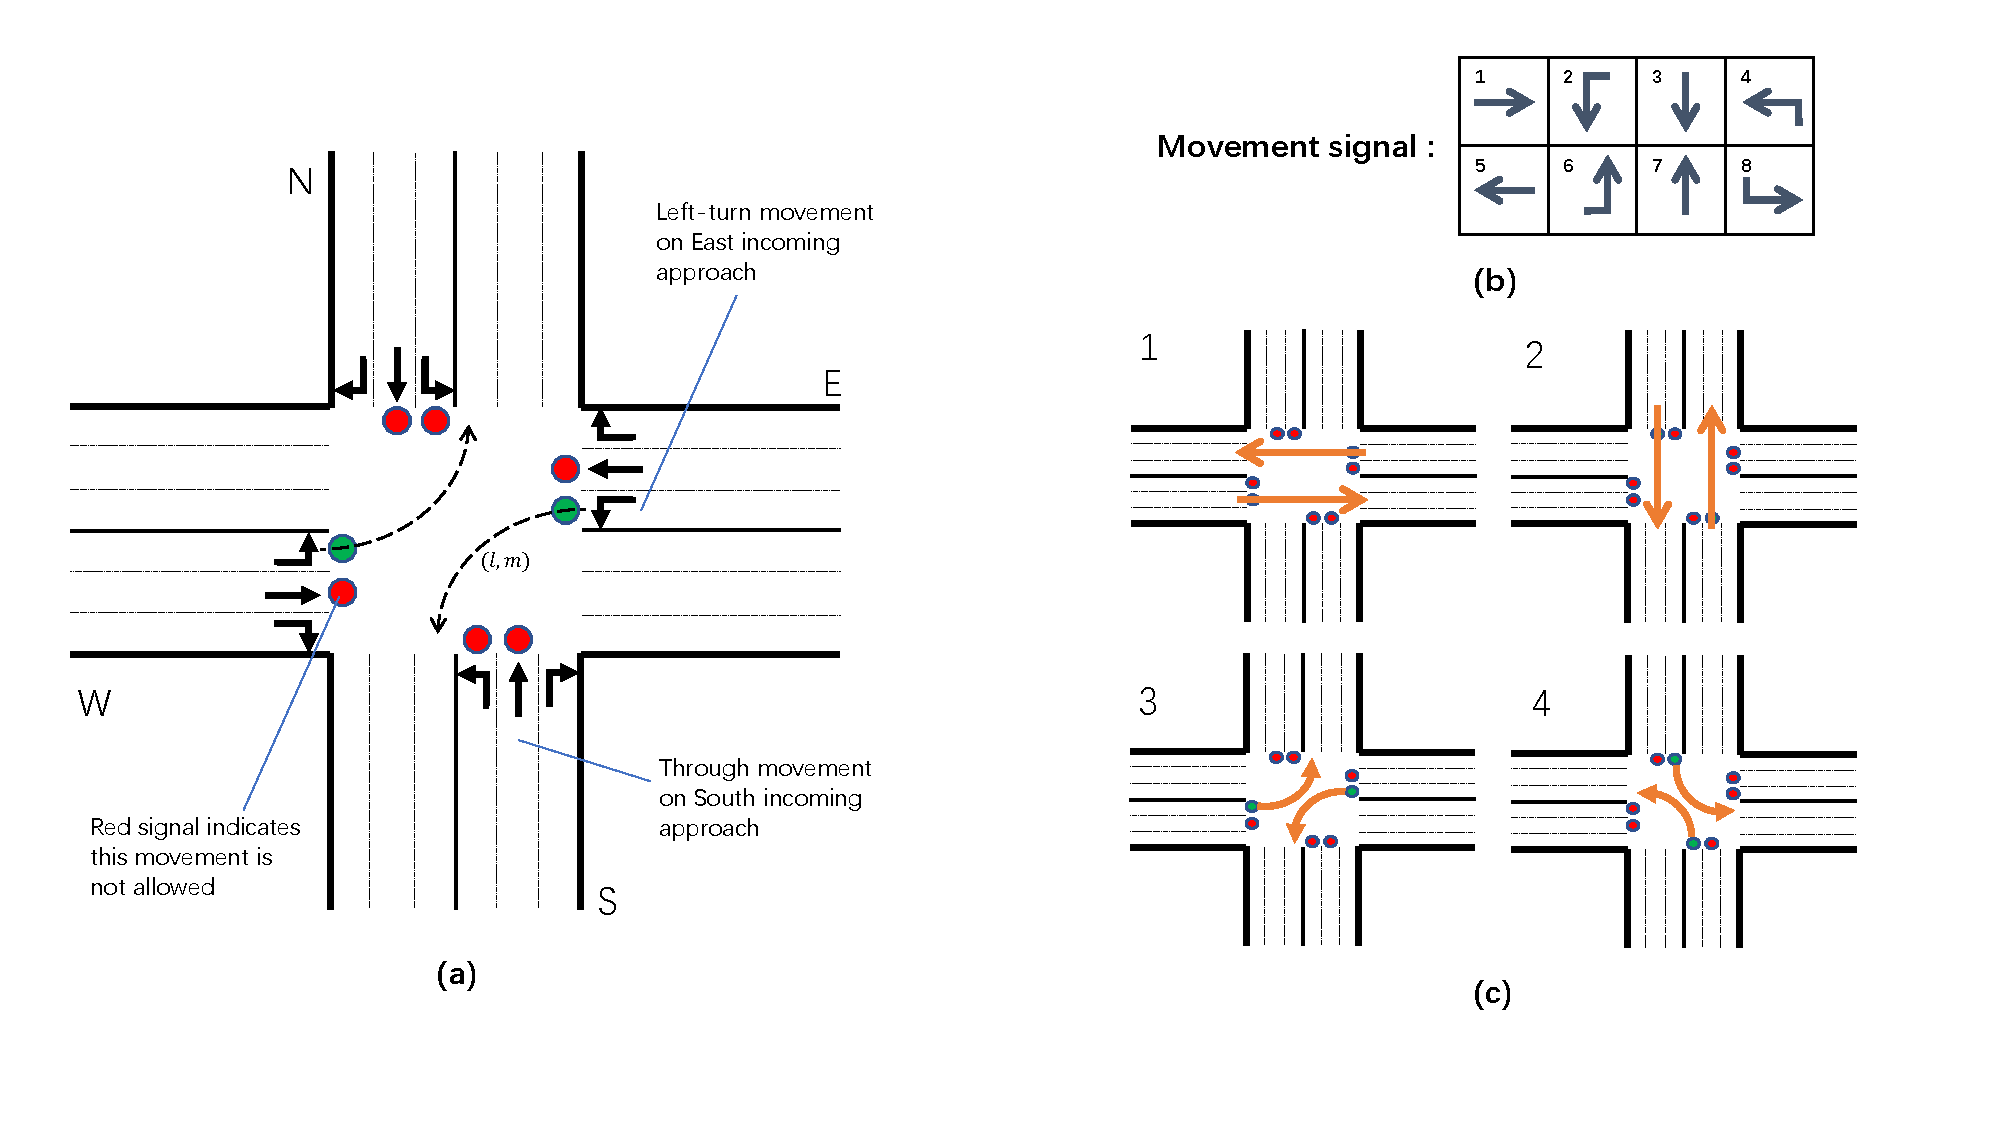
\includegraphics[width=.9\textwidth]{fig/tsc.pdf}
    \caption{tsc}
    \label{fig:tsc}
\end{figure}
\section{基本术语}
\begin{itemize}
    \item Approach: 指交叉路口的巷道。任何一个交叉路口都有两种approach,进入路口的incoming approach和离开路口的outgoing approach。\autoref{fig:tsc}(a)描述了一个典型的有8个approach(四个入口,四个出口)的交叉路口。
    \item Lane:一个Approach是由一组车道组成。与Approach的定义类似,车道也分为两种:转入车道(incoming lane)和转出车道(outgoing lane)。
    \item Traffic movement:指的是车流从一个incoming approach 运动到另一个outgoing approach,表示为$\left(r_{i}, r_{o}\right)$,其中ri和ro分别表示incoming lane和outgoing lane。通常,traffic movement可以分为左转、直行以及右转三种,在少数特殊的路口也支持U-turn的traffic movement。
    \item Movement signal:根据traffic movement定义的运动信号,绿色代表可以通行,红色代表禁止通行。根据大多数国家的交通规则,右转的traffic movement是可以不受信号约束的。
    \item Phase: 信号灯的一个phase(相位)是指非冲突运动信号的组合,这意味着这些信号可以同时设置为绿色,而不会引起安全冲突。 \autoref{fig:tsc}(c)展示了最常用的四相位信号模式。
    \item Phase sequence: 相序,即一组相位的序列,它定义了一组相位及其变化顺序。
    \item Signal plan:信号计划,由一组相位序列及其相应的起始时间组成。通常表示为$\left(p_{1}, t_{1}\right)\left(p_{2}, t_{2}\right) \ldots\left(p_{i}, t_{i}\right) \ldots$其中$p_{i}$ 和 $t_{i}$分别代表相位及其开始时间。
    \item Cycle-based signal plan:周期性信号计划,与普通的信号计划不同的是其中的相位序列是按循环顺序工作的,可以表示为
    $\left(p_{1}, t_{1}^{1}\right)\left(p_{2}, t_{2}^{1}\right) \ldots \\ \left(p_{N}, t_{N}^{1}\right)\left(p_{1}, t_{1}^{2}\right)\left(p_{2}, t_{2}^{2}\right) \ldots\left(p_{N}, t_{N}^{2}\right) \ldots$,其中$p_{1}, p_{2}, \ldots, p_{N}$是重复出现的相位序列,$t_i^j$是$j$周期中相位$p_i$的起始时间。具体地,$C^{j}=t_{1}^{j+1}-t_{1}^{j}$是第j周期的周期长度, $\left\{\frac{t_{2}^j-t_{1}^j}{C^j}, \ldots, \frac{t_{N}^j-t_{N-1}^j}{C^j}\right\}$是第$j$周期中的相位分裂比(phase split ratio),表示每个相位持续时间占总周期长度的比重。现有的交通信号控制方法通常在一天中重复类似的相位序列。
\end{itemize}


\section{传统交通控制方法}
\subsection{Fixed-Time}
使用最为广泛的一种交通信号控制方法,按照事先固定的信号序列不断的循环,不依赖于任何类型的检测,例如行人按钮或车辆检测装置。所有道路和运动都以恒定的特定顺序提供服务。即使没有汽车或行人,信号也会改变,在交通较为稳定的情况下能够起到不错的效果,但是当交通变化很大时效率会很低。由于不需要安装任何检测器,所以这种方法的成本效益高。

\subsection{Webster}
对于单个交叉口,交通运输工程领域中的交通信号控制方法通常由三个部分组成:确定信号周期长度,确定信号相位序列以及相位分裂。Webster是一种广泛使用的计算单个交叉路口的信号周期长度和相位分裂时间的方法。通过假设车流在一段时间内(例如,过去的五分钟或10分钟)是均匀到达的,可以计算出确切的最优周期和最佳相位分裂时间,从而最小化车量通行时间。

\subsection{GreenWave}
虽然使用Webster可以简单的控制单个交叉路口的交通信号,但是对于相邻的多个交叉路口,不能够简单地直接使用Webster来分别优化每一个路口,相邻路口信号灯的信号时间之间的偏移(即相邻路口信号周期起始时间的差值)也需要进行优化,因为对于相距较近的路口来说,一个路口的控制策略可能会影响到其他路口。
GreenWave就是交通运输领域中最经典的协调相邻路口的信号控制方法,它通过优化相邻路口信号时间的偏移来减少车辆在某一方向行驶时的停留次数。其中路口之间的偏移量通过以下公式计算:
\begin{align}
    \label{eq:green-wave}
    \Delta t_{i, j}=\frac{L_{i, j}}{v}
\end{align}
其中$L_{i, j}$是路口$i$和路口$j$之间的道路长度,$v$是道路上车辆的预期行驶速度。这种方法可以形成沿指定交通方向的绿色信号波,在该方向行驶的车辆可以受益于渐进的绿色信号级联,而不会在任何交叉口停留,如下图所示:
\begin{figure}[htb]
    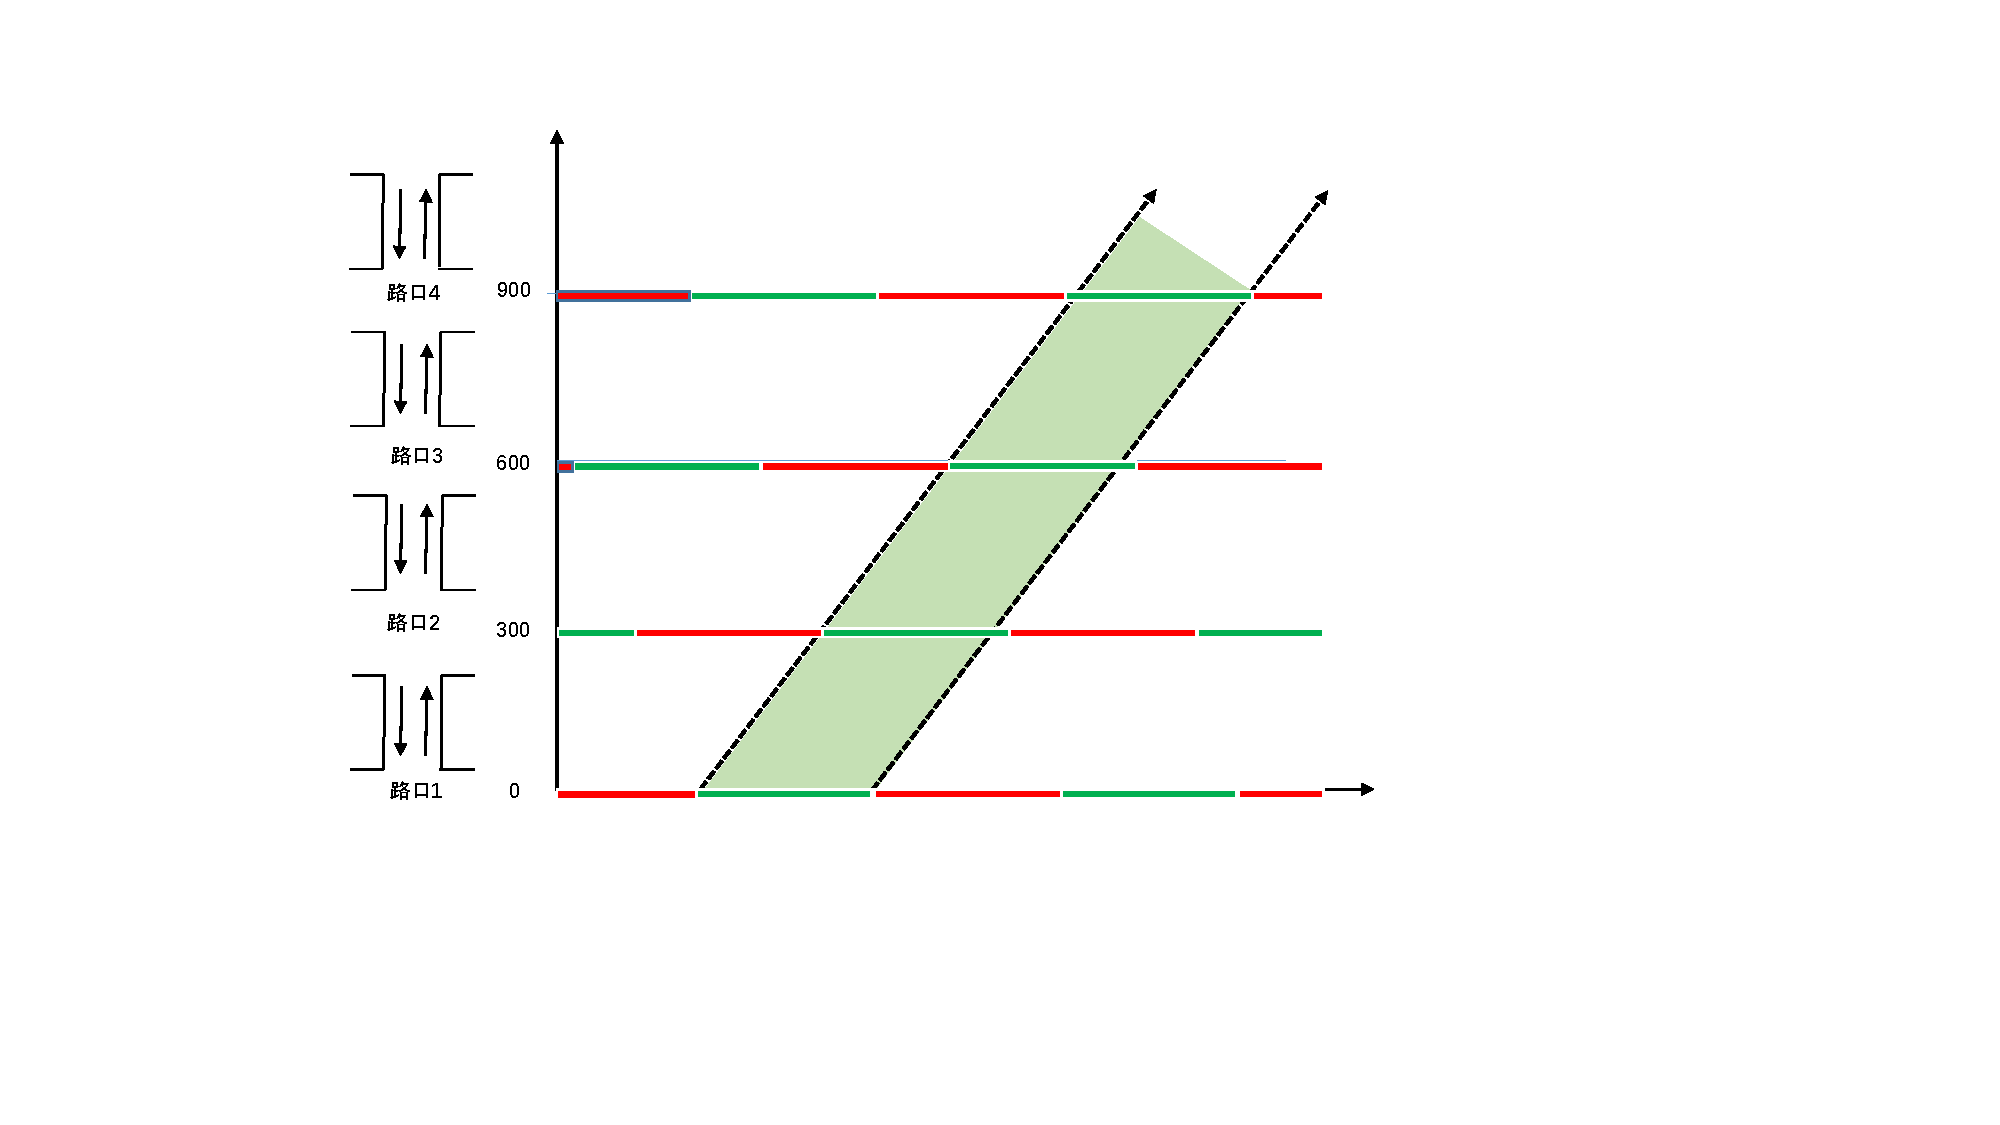
\includegraphics[width=1.2\textwidth]{fig/green-ware.pdf}
    \caption{green-wave}
    \label{fig:green-wave}
\end{figure}

\subsection{Actuated Control}
Actuated Control根据当前信号相位和其他的竞争信号相位对绿色信号的请求来决定是否保持或者变化当前的相位。请求触发规则如下:
\begin{itemize}
    \item 1. 当目前信号相位的持续时间未达到最小时间周期时,或在当前相位对应入车道上有车辆进入,并且在接近信号的距离内时,就会产生延长绿色信号时间的请求,以让车辆可以直接通过路口。 
    \item 2. 当竞争信号相位的等待车辆数量大于一个阈值时,就会生成对绿色信号的请求。
\end{itemize}
根据规则的差异,Actuated Control主要可以分为Fully-Actuated Control和Semi-Actuated Control两种。

\subsection{SOTL}
Self-Organizing Traffic Light Control(SOTL)是一种具有附加需求响应规则的Fully-Actuated Control方法。它与Fully-Actuated Control的主要区别在于当前信号相位的绿色信号请求定义(虽然它们都需要最小的绿色相位持续时间),在Fully-Actuated Control中,当车辆接近信号灯时,就会产生延长绿色信号的请求,而在SOTL中,除非接近信号灯的车辆数量大于预先定义的一个阈值,否则就不会产生绿色信号请求。

\subsection{Max-Pressure Control}
Max-Pressure Control的目的是通过最小化对应信号相位的压力(pressure)来平衡相邻路口之间的队列长度,从而降低过饱和的风险,其中压力的概念如图\autoref{fig:max-pressure}所示:
\begin{figure}[htb]
    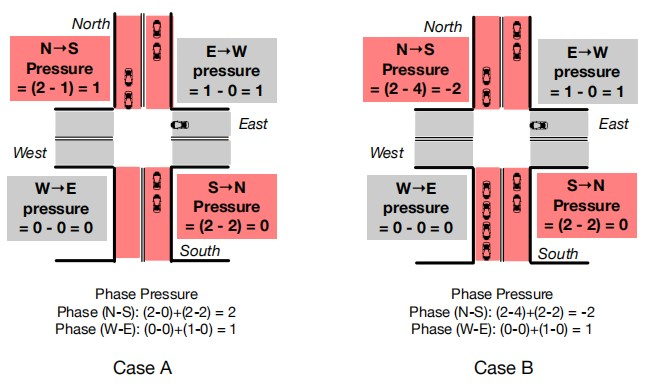
\includegraphics[width=0.9\textwidth]{fig/max-pressure.jpg}
    \caption{Max-Pressure的压力图示}
    \label{fig:max-pressure}
\end{figure}
其中运动信号的压力是指转入车道上的车辆数减去相应的转出车道上的车辆数,而信号相位的压力定义为转入巷道和转出巷道上的总队列长度之间的差异。Varaiya\cite{varaiya2013max}等人证明了当将优化目标设为最小化单个路口的相位压力时,Max-Pressure Control可以最大限度地提高真个路网的吞吐量。

\autoref{tab:traditional-methods}列出了每种方法的要求和输出结果:
\begin{table}[htb]
    \caption{传统交通信号控制方法总结\label{tab:traditional-methods}}
    \begin{tabular}{llll}
      \toprule
      方法 & 先验信息 & 输入 & 输出 \\
      \midrule
      Webster & 相位序列 & 交通流量 & 基于周期的单个路口信号计划 \\
      GreenWave & 信号计划 & 交通流量、速度限制、车道长度 & 基于周期的信号计划的偏移量 \\
      Actual Control, SOTL & 相位序列& 交通流量 & 是否变化到下一个相位\\
      Max-Pressure Control & 无 & 队列长度 & 所有交叉口的信号计划\\
      \bottomrule
    \end{tabular}
\end{table}

\section{基于强化学习的交通信号控制}
最近,人们提出了不同的人工智能技术来控制交通信号,例如遗传算法、群体智能以及强化学习。 其中在这些技术中,强化学习在近年来更具趋势。
\subsection{强化学习概述}
\begin{figure}[htb]
    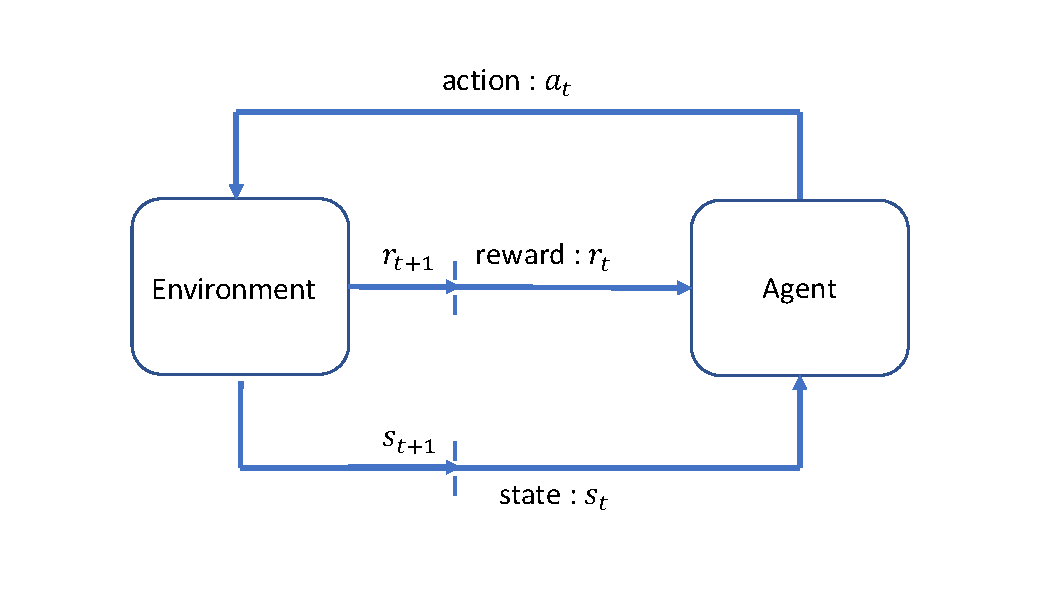
\includegraphics[width=10cm]{fig/rl.pdf}
    \caption{马尔可夫决策过程}
    \label{fig:mdp}
\end{figure}
通常单智能体强化学习问题被建模成马尔可夫决策过程(Markov Decision Process, MDP, 如\autoref{fig:mdp}所示) $<\mathcal{S}, \mathcal{A}, P, R, \gamma>$,其中$\mathcal{S}, \mathcal{A}, P, R, \gamma$分别表示状态集、动作集、概率状态转移函数、奖励函数和折扣因子。具体定义如下:
\begin{itemize}
    \item $\mathcal{S}$:在时间步骤$t$,智能体得到一个观测状态$s^t \in \mathcal{S}$。
    \item $\mathcal{A}, P$:在时间步骤$t$,智能体采取一个动作$a^t \in \mathcal{A}$,然后环境根据状态转移函数转移到一个新的状态。
    \begin{align}
        P\left(\mathrm{~s}^{t+1} \mid \mathrm{s}^{t}, \mathrm{a}^{t}\right): \mathcal{S} \times \mathcal{A} \rightarrow \mathcal{S}
    \end{align}
    \item $R$:在时间步骤$t$,智能体通过奖励函数获得一个奖励$r^t$。
    \begin{align}
        R\left(s^{t}, a^{t}\right): \mathcal{S} \times \mathcal{A} \rightarrow \mathbb{R}
    \end{align}
    \item $\gamma$:智能体的目标是找到一种使预期收益最大化的策略,即累积(折扣)奖励之和。折扣因子决定了即时奖励与未来奖励的重要性。
    \begin{align}
        G^{t}:=\sum_{i=0}^{\infty} \gamma^{i} r^{t+i}
    \end{align}
  \end{itemize}
通常解决一个强化学习任务意味着要找到一个能够使预期收益最大化的最优策略$\pi^*$,一般来说,我们难以直接找到这个最优策略,更多的是比较若干个不同的策略然后从中选出较好的那个作为局部最优解。而策略的筛选是通过比较其对应的价值函数来实现的,即通过寻找较优的价值函数来筛选出较优的策略。价值函数是对未来奖励的期望,根据输入的不同可以分为状态价值函数和动作价值函数。
状态价值函数的定义如下:
\begin{align}
    V_{\pi}(s)=\mathbb{E}_{\pi}\left[G_{t} \mid S_{t}=s\right]
\end{align}
其描述的是当在$t$时刻处于状态$s$的预期收益。动作价值函数的定义如下:
\begin{align}
    Q_{\pi}(s, a)=\mathbb{E}_{\pi}\left[G_{t} \mid S_{t}=s, A_{t}=a\right]
\end{align}
其描述的是当在状态$s$下采取动作$a$的预期收益。

最优策略$\pi^{*}$对应的是最优状态价值函数和最优动作价值函数。最优状态价值函数定义为$V_{\pi}^*(s)=\mathcal{max}_{\pi}V^{\pi}(s)$,它满足以下贝尔曼最优方程:
\begin{align}
    V^{*}\left(\mathrm{~s}^{t}\right)=\max _{\mathrm{a}^{t} \in \mathcal{A}} \sum_{\mathrm{s}^{t+1} \in \mathcal{S}} P\left(\mathrm{~s}^{t+1} \mid \mathrm{s}^{t}, \mathrm{a}^{t}\right)\left[\mathrm{r}+\gamma v_{*}\left(\mathrm{~s}^{t+1}\right)\right], \forall \mathrm{s}^{t} \in \mathcal{S}
\end{align}
最优动作价值函数定义为$Q^*(s,a)=\mathcal{max}_{\pi}Q^{\pi}(s,a)$,其满足以下贝尔曼最优方程:
\begin{align}
    Q^{*}\left(s^{t}, a^{t}\right)=\sum_{s^{t+1} \in \mathcal{S}} P\left(s^{t+1} \mid s^{t}, a^{t}\right)\left[r^{t}+\gamma \max _{a^{t+1}} Q^{*}\left(s^{t+1}, a^{t+1}\right)\right], \forall s^{t} \in \mathcal{S}, a^{t} \in \mathcal{A}
\end{align}

\subsubsection{分类}
\begin{figure}[htb]
    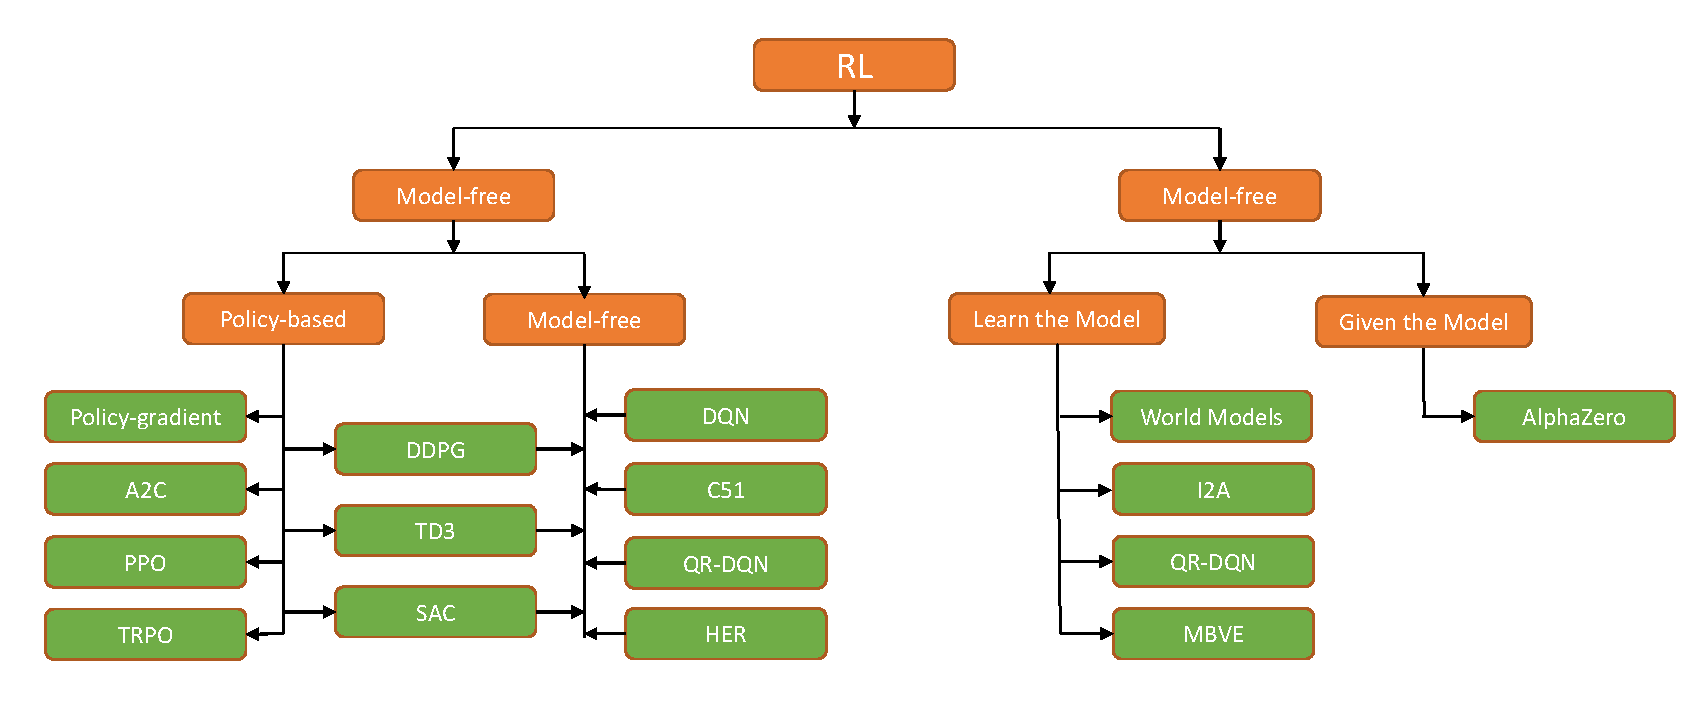
\includegraphics[width=0.9\textwidth]{fig/rl-classfication.pdf}
    \caption{强化学习分类及常见算法}
    \label{fig:rl-classficatoin}
\end{figure}
强化学习主要可以分为两大类:Model-based(有模型)和Model-free(无模型)。其中Model-based又可以分为基于策略函数(Policy-based)和值函数(Value-based)两大类,而Model-free可以分为模型学习(Learn the Model)和给定模型(Given the Model)两大类,具体如\autoref{fig:rl-classficatoin}所示。

Model-free方法是指在不知道状态转移函数函数的情况下,通过采样大量的经验来学习策略函数(Policy Function)或者价值函数(Value函数)。其中Policy-based的方法直接将拟学习的策略参数化,在以最大化奖励的目标下,直接对策略函数进行优化。而Value-based的方法则是学习一个最佳策略对应的动作价值函数的近似。当然,Policy-based和Value-based并非无法兼容的,有一类方法(Actor-Critic)就是融合了两中方法的思想。
这类方法同时使用策略和价值评估来做出决策,其中,智能体会根据策略做出动作,而价值函数会对做出的动作给出评分,这样可以在原有的基于策略的方法的基础上加速学习过程,取得更好的效果。代表算法如\autoref{fig:rl-classficatoin}中的DDPG\cite{lillicrap2015continuous}、TD3\cite{fujimoto2018addressing}以及SAC\cite{haarnoja2018soft}等。

Model-based方法是指在已知状态转移函数的情况下,学习用一个模型去模拟环境,然后用这个模拟的环境去预测接下来可能会发生的所有所有情况并从中选择最有利的情况。

% 根据是否有学习环境模型可以分为:
% \begin{itemize}
%     \item Model-based:指在已知状态转移分布条件下,智能体根据这个模型做出预先设定好的决策。通常意义来讲,动态规划是一种有模型的强化学习算法。
%     \item Model-free:指在未知状态转移分布条件下,通过学习价值函数(Value Function)和策略函数(Policy Function)进行决策,通常需要大量的采样来估计状态、动作及反馈函数,从而优化动作策略。
% \end{itemize}
% 根据学习目标可以分为:
% \begin{itemize}
%     \item Value-based:这类方法的目标是学习价值函数,只能应用在不连续的、离散的环境下(如围棋或某些游戏领域),对于行为集合规模庞大、动作连续的场景(如机器人控制领域),其很难学习到较好的结果。代表算法有Q-learning\cite{watkins1992q},DQN\cite{mnih2015human}等。
%     \item Policy-based:这类方法直接对策略进行优化,使制定的策略能够获得最高的反馈。代表算法有Policy Gradient\cite{sutton2000policy}算法等。
%     \item Actor-Critic:这类方法同时使用策略和价值评估来做出决策,其中,智能体会根据策略做出动作,而价值函数会对做出的动作给出评分,这样可以在原有的基于策略的方法的基础上加速学习过程,取得更好的效果。代表算法有A2C\cite{barto1983neuronlike}等。
% \end{itemize}



\subsection{基于强化学习的交通信号控制框架}
\begin{figure}[t]
    \label{fig:TSC-RL}
    \subfloat[单路口场景\label{fig:single-tsc-rl}]{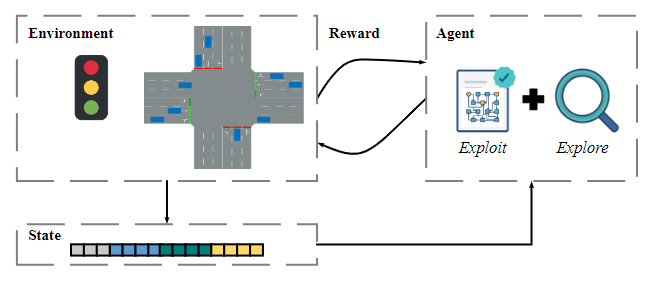
\includegraphics[width=0.45\textwidth]{./fig/single-intersection-RL.PNG}}\quad
    \subfloat[多路口场景\label{fig:multi-tsc-rl}]{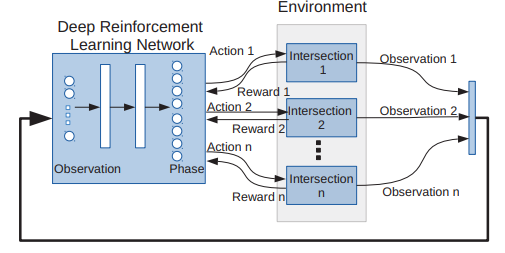
\includegraphics[width=0.45\textwidth]{./fig/multi-intersection-RL.PNG}}
    \caption[]{基于强化学习的交通信号控制框架}
  \end{figure}
根据路网规模的不同,基于强化学习的交通信号控制框架可以分为以下两类:
\begin{itemize}
    \item 单路口交通信号控制:\autoref{fig:single-tsc-rl}描述了应用强化学习框架到单路口交通信号控制问题上的基本思路。环境是道路上的交通状况,智能体要做的是控制交通信号。在每个调度时刻$t$,获取环境的状态描述$s^t$(例如,当前的信号相位,车辆的等待时间,排队长度,车辆的位置),智能体将根据这个状态描述对下一步采取的行动作出预测,以使预期收益最大化,然后该动作将在环境中执行,并且产生一个奖励$r^t$。通常,在决策过程中,智能体采取的策略结合了对所学策略的利用和对新策略的探索。
    \item 多路口交通信号控制:\autoref{fig:multi-tsc-rl}描述了应用强化学习框架到多路口交通信号控制问题上的基本思路。智能体被定义为环境中N个路口的信号控制者。目标是学习每个智能体的最优策略,以优化整个环境中所有路口的通行效率。在每个调度时刻$t$,每个智能体$i$观察环境的一部分作为观察点$o_i^t$。智能体将对接下来要采取的行动$\mathbf{\alpha}^t$做出预测。这些动作将在环境中执行,并产生奖励$r_i^t$,其中奖励可以在环境中的单个路口或一组路口的层面上定义。
\end{itemize}
\subsection{基本要素}
使用强化学习来解决交通信号控制问题要先确定以下几个基本要素:

\textbf{奖励设计}:由于强化学习是以最大化累计奖励为目标来学习的,所以奖励的选择决定了学习的方向。在交通信号控制问题中,虽然最终目标是尽量减少所有车辆的通行时间,但由于几个原因,通行时间很难直接作为RL的有效奖励。首先,车辆的行驶时间不仅受交通信号灯的影响,还受车辆自由流动速度等其他因素的影响。其次,当交通信号控制器事先不知道车辆行驶目的地(在现实世界中往往是这样),优化道路上所有车辆的通行时间变得特别困难。 在这种情况下,车辆的通行时间只能在多个动作完成后车辆完全离开路口后才能测量。已有工作的奖励设计通常是基于一些可以直接在一个动作后测量的指标的加权和。例如,等待车辆的队列长度、车辆等待时间、速度、累计延迟、路口的吞吐量、车辆平均停车次数、信号变化频率(信号在一定时间段内变化的次数,学习到的策略不应该太过频繁的改变信号)以及路口的压力(Max-pressure中定义的pressure)等。虽然将奖励定义为几个因素的加权线性组合是现有研究中的一种常见做法,并且取得了不错的效果,但是这种特别的设计存在两个问题。第一,无法保证最大化设计的奖励等价于最优的通行效率,因为它们在交通运输理论中没有直接联系。第二,调整每个奖励函数因子的权重是相当棘手的,在权重设置上的微小差异可能会导致最终的结果有显著的差别。

\textbf{状态表示}:状态表示是以一种数值化的形式来描述路口的交通状况,描述的越全面越有利于快速学习到最优策略,通常使用多个要素组合来描述交通状况,例如,队列长度、车辆等待时间、车辆数量(包含非等待车辆),车辆速度、车辆位置分布以及当前信号灯的相位等。最近,在基于RL的交通信号控制算法中出现了使用更复杂状态的趋势,希望能够更全面地描述交通状况。 Mousavi、Van derPol以及Wei Hua等人在他们的研究工作中提出使用位置图片来当作状态描述。但是,具有如此高维度的状态学习往往需要大量的训练样本,这意味着训练RL智能体需要很长时间。 更重要的是,较长的学习进度不一定会导致显著的性能增益,因为智能体可能需要花费更多的时间从状态表示中提取有用的信息。因此,状态的表示应该简洁且能够充分地描述环境。

\textbf{动作选择机制}:动作选择机制决定了以何种方式来控制信号灯,不同的动作机制有不同的影响。主要可以总结为以下四种方式:
\begin{itemize}
    \item 确定当前相位时长:在这中动作选择机制下,智能体学习通过从预定义的候选时间段(比如,10秒、15秒、20秒等)中选择来设置当前相位的持续时间。
    \item 确定基于周期的相位比:这种方式定义的动作为下一个周期的相位分裂比(phase split ratio) 通常,给出总周期长度,并预先定义一个包含一些相位比的候选集。
    \item 保持或改变当前相位:这种方式也是基于周期性的信号计划,通常一个二进制数来定义动作。例如,1表示保持当前相位,0表示变换到下一相位。
    \item 选择下一个相位:这种方式直接从待选相位序列中选择一个相位并变化到该相位,其中相位序列不是预定的。因此,这种信号控制方式更加的灵活,智能体学习在不同的而状态下选择最优的相位,而不假设信号会以循环的方式改变。
\end{itemize}

% \textbf{学习算法}:强化学习发展至今已经提出了很多不同的算法,根据估计潜在奖励和选择动作的不同可以分为以下两种:
% \begin{itemize}
%     \item Value-based Methods:基于值的方法的目标近似于状态-值函数或状态-动作值函数,策略是从学习的值函数隐式获得的。基于于价值的方法(Q-learning和DQN等), 直接模拟状态价值函数或状态动作价值函数(例如,在当前交通情况下,如果进行一个动作,平均速度的增加/减少将生效多少?)。 这样,状态和奖励就可以直接输入模型,而不需要额外的处理。 然而,这些方法通常与$\epsilon-greedy$的动作选择机制相结合,因此当$\epsilon$最终衰减到一个很小的数目时,将导致一个几乎确定性的策略(即,在某些状态下的动作是确定性的)。 这可能会导致智能体陷入一些看不见的或代表性不足的情况,而没有改进。 此外,这些方法只能处理离散的动作,因为它需要对每个动作进行单独的建模过程。
%     \item Policy-based Methods:基于策略的方法直接更新策略(例如,在特定状态下采取行动的概率向量)参数,以最大限度地实现预定目标(例如平均预期回报)。 基于策略的方法,尝试学习某一状态下不同动作的概率分布。 基于政策的方法的优点是,它不要求行动是离散的。 此外,它可以学习一个随机策略,并继续探索潜在的更有价值的行动。Actor-Critic基于策略的方法中广泛使用的框架之一。 它包括基于价值的思想来学习行动概率分布的策略,Actor控制我们的智能体的行为(policy-based),Critic衡量所采取的行动有多好(value-based)。 Aslani\cite{aslani2019developing,aslani2017adaptive}、Mousavi\cite{mousavi2017traffic}以及Prashanth\cite{prashanth2011reinforcement}在他们的工作中使用Actor-Critic,利用价值函数逼近和策略优化的优势,在交通信号控制问题上表现出优异的性能。
% \end{itemize}

\section{图神经网络}
由于我们的工作中涉及到图神经网络的知识,这里给出一些有关图神经网络的简单描述。
\subsection{图神经网络概述}

深度网络的研究推进了模式识别和数据挖掘领域的发展。借助于计算资源的高速发展(如GPU),深度学习在欧几里得数据(如图像、文本和视频)中取得巨大的成功。但是在一些应用场景下,数据(图)是由非欧几里得域生成的,任然需要有效分析。
例如,在电子商务领域,一个基于图的学习系统能够利用用户和商品之间的交互以实现精准的推荐。在化学领域,分子被建模为图,新药研发需要测定其生物活性。在论文引用网络中,论文之间通过引用关系互相连接,需要将它们分成不同的类别。

图数据的复杂性对现有机器学习算法提出了巨大的挑战,因为图数据是不规则的。每张图大小不同、节点无序,一张图中的每个节点都有不同数目的邻近节点,使得一些在图像中容易计算的重要运算(如卷积)不能再直接应用于图。此外,现有机器学习算法的核心假设是实例彼此独立。
然而,图数据中的每个实例都与周围的其它实例相关,含有一些复杂的连接信息,用于捕获数据之间的依赖关系,包括引用、朋友关系和相互作用。最近,越来越多的研究开始将深度学习方法应用到图数据领域。受到深度学习领域进展的驱动,研究人员在设计图神经网络的架构时借鉴了卷积网络、循环网络和深度自编码器的思想。

图神经网络的概念最早由Gori\cite{gori2005new}等人提出,由Scarselli\cite{scarselli2008graph}等人进一步阐明。早期的初期是以迭代方式通过循环神经网络架构传播邻近信息来学习目标节点的表示,直至达到稳定的状态。

图神经网络可以分为:图卷积网络(Convolutional graph neural networks),图注意力网络(Graph Attention Network),图自编码器(Graph Auto-encoder),图生成网络(Graph Generative Network)和图时空网络(Graph Spatial-Temporal Network)。

\subsection{图卷积网络}
图卷积网络是将卷积运算从传统数据(如图片、视频)推广到了图数据上的模型,如\autoref{fig:GCN}所示。其主要思想是通过聚合节点$v$自身的特征和邻居节点的特征来生成节点$v$的表示。图卷积网络在构建许多其他的图神经网络模型方面发挥了重要作用。
\begin{figure}[htb]
    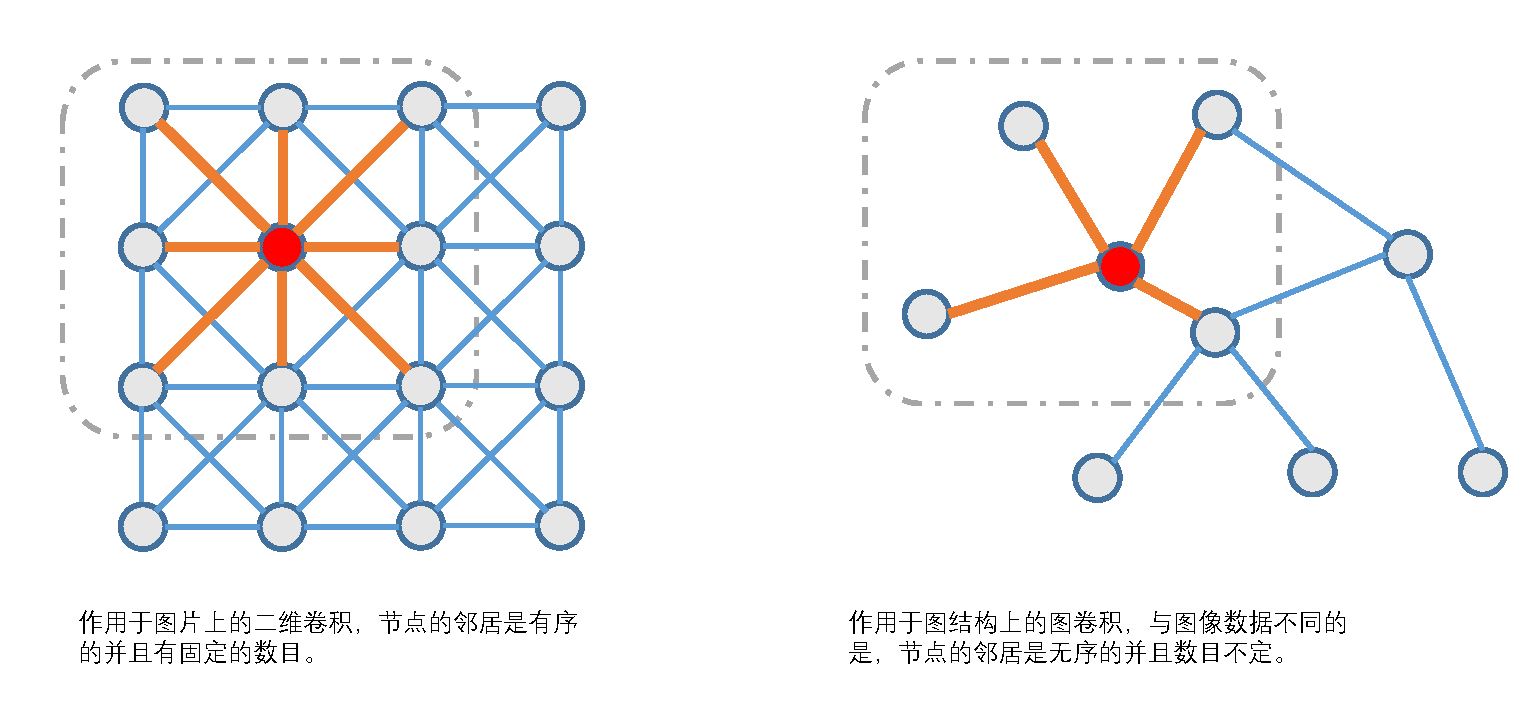
\includegraphics[width=1.2\textwidth]{fig/GCN.pdf}
    \caption{图卷积示意图}
    \label{fig:GCN}
  \end{figure}
图卷积网络按照卷积的方式可以分为两类:基于谱(spectral-based)和基于空间(spatial-based)的方法。基于谱的方法从信号处理的角度引入滤波器来定义图卷积 [82],其中图卷积操作被解释为从图信号中去除噪声。基于空间的方法则是通过信息传播来定义图卷积。

\subsection{图注意力网络}
图注意力网络是将注意力机制引入到基于空间域的图神经网络。图神经网络不需要使用拉普拉斯等矩阵进行复杂的计算,仅通过邻居节点的表征来更新目标节点的特征。由于能够放大数据中最重要部分的影响,注意力机制已经广泛应用到很多基于序列的任务中,图神经网络也受益于此,在聚合过程中使用注意力整合多个模型的输出。主要方法包括:
\begin{figure}[htb]
    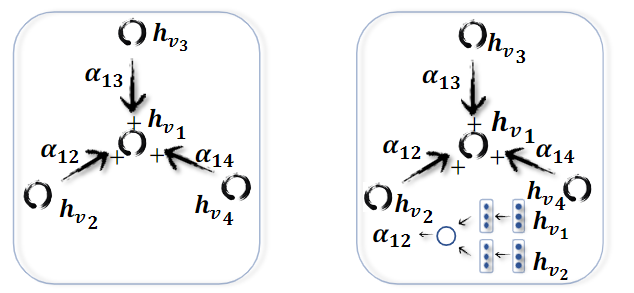
\includegraphics[width=1.2\textwidth]{fig/gcn-gat.png}
    \caption{GCN与GAT聚合信息的区别}
    \label{fig:GCN-GAT}
  \end{figure}
\begin{itemize}
    \item Graph Attention Network(GAT)\cite{velivckovic2017graph}:本质上GAT是一种基于空间的图卷积网络,它与GCN的主要区别在于对邻居节点信息的聚合方式不同(\autoref{fig:GCN-GAT})。GCN在在聚合过程中显式地为节点$v_i$的邻居$v_j$赋予一个非参数静态权重$a_{ij}=\frac{1}{\sqrt{\operatorname{deg}\left(v_{i}\right) \operatorname{deg}\left(v_{j}\right)}}$。而GAT则是通过使用一个端到端的神经网络架构隐式地捕捉权重$a_{ij}$,以便更重要的节点获得更大的权重,具体操作如下:
    \begin{align}
        \mathbf{h}_{i}^{t}=\sigma\left(\sum_{j \in \mathcal{N}_{i}} \alpha\left(\mathbf{h}_{i}^{t-1}, \mathbf{h}_{j}^{t-1}\right) \mathbf{W}^{t-1} \mathbf{h}_{j}^{t-1}\right),
    \end{align}
    其中$\alpha(\cdot)$是一个注意力函数,它可以动态地调整邻居节点$j$对目标节点$i$的贡献。通常为了学习不同子空间中的注意力权重,GAT会使用多个注意力函数(即多头注意立机制,Multi-head Attention):
    \begin{align}
        \mathbf{h}_{i}^{t}=\|_{k=1}^{K} \sigma\left(\sum_{j \in \mathcal{N}_{t}} \alpha_{k}\left(\mathbf{h}_{i}^{t-1}, \mathbf{h}_{j}^{t-1}\right) W_{k}^{t-1} \mathbf{h}_{j}^{t-1}\right),
    \end{align}

    \item Gated Attention Network(GAAN)\cite{lee2017deep}\cite{zhang2018gaan}:GAAN除了采用多头注意力机制(self-attention mechanism)外,还引入了自注意机制来更新节点的隐藏状态。自注意机制可以为每个注意力头计算出一个额外的注意分数:
    \begin{align}
        \mathbf{h}_{i}^{t}=\phi_{o}\left(\mathbf{x}_{i} \oplus \|_{k=1}^{K} g_{i}^{k} \sum_{j \in \mathcal{N}_{\mathbf{t}}} \alpha_{k}\left(\mathbf{h}_{i}^{t-1}, \mathbf{h}_{j}^{t-1}\right) \phi_{v}\left(\mathbf{h}_{j}^{t-1}\right)\right),
    \end{align}
    其中$\phi_{o}\text{和}\phi_{v}$是反馈神经网络,而$g_{i}^{k}$是第$k$个注意力头的权重。
    \item Graph Attention Model(GAM):GAM是一种用来解决图形分类问题的循环神经网络模型。它可以通过自适应地访问某个重要节点的序列来对图的信息进行处理,其模型定义如下:
    \begin{align}
        \mathbf{h}_{t}=\mathbf{f}_{h}\left(\mathbf{f}_{s}\left(\mathbf{r}_{t-1}, \mathbf{v}_{t-1}, g ; \theta_{s}\right), \mathbf{h}_{t-1} ; \theta_{h}\right),
    \end{align}
    其中$\mathbf{f}_{h}(\cdot)$是一个LSTM网络,$f_s$是一个step network,它会优先访问当前节点$v_{t-1}$优先级高的邻居并将它们的信息进行聚合。
\end{itemize}
\subsection{图自编码器}
图自编码器是一类图嵌入方法,其目的是利用神经网络将图的顶点表示为低维向量。典型的解决方案是利用多层感知机作为编码器来获取节点嵌入,其中解码器重建节点的邻域统计信息,如positive pointwise mutual information (PPMI)或一阶和二阶近似值。
主要包括基于GCN的自编码器,如Graph Autoencoder(GAE)\cite{kipf2016variational}和Adversarially Regularized Graph Autoencoder (ARGA)\cite{pan2018adversarially},以及Network Representations with Adversarially Regularized Autoencoders (NetRA)\cite{yu2018learning}、Deep Neural Networks for Graph Representations (DNGR)\cite{cao2016deep}、Structural Deep Network Embedding (SDNE)\cite{wang2016structural}和Deep Recursive Network Embedding (DRNE)\cite{tu2018deep}。
DNGR和SDNE学习仅给出拓扑结构的节点嵌入,而GAE、ARGA、NetRA、DRNE用于学习当拓扑信息和节点内容特征都存在时的节点嵌入。图自动编码器的一个挑战是邻接矩阵A的稀疏性,这使得解码器的正条目数远远小于负条目数。为了解决这个问题,DNGR重构了一个更密集的矩阵,即PPMI矩阵,SDNE对邻接矩阵的零项进行惩罚,GAE对邻接矩阵中的项进行重加权,NetRA将图线性化为序列。
\subsection{图生成网络}
图生成网络的目标是在给定一组观察到的图的情况下生成新的图。图生成网络的许多方法都是特定于领域的。例如,在分子图生成中,一些工作模拟了称为SMILES的分子图的字符串表示。在自然语言处理中,生成语义图或知识图通常以给定的句子为条件。这种方法通常使用GCN或者其他框架作为基础构建模块,其中使用GCN构建的方法有:
\begin{itemize}
    \item Molecular Generative Adversarial Networks (MolGAN)\cite{de2018molgan}:MolGAN整合了图卷积网络、图注意力网络和强化学习以生成具有预期属性的图。MolGAN由生成器和判别器组成,相互竞争以提高生成器的真实性。在MolGAN中,生成器尝试提出一个假图及其特征矩阵,而鉴别器旨在将假样本与经验数据区分开来。此外,还引入了一个奖励网络来促使生成器能够按照外部的评估生成具有特定属性的图。
    \item Deep Generative Models of Graphs (DGMG)\cite{li2018learning}:利用基于空间的图卷积网络来获得现有图的隐藏表示。生成节点和边的决策过程是以整个图的表示为基础的。简而言之,DGMG递归地在一个图中产生一个节点,直到达到某个停止条件。在添加新节点后的每一步,DGMG都会反复决定是否向添加的节点添加边,直到决策的判定结果变为假。如果决策为真,则评估将新添加节点连接到所有现有节点的概率分布,并从概率分布中抽取一个节点。将新节点及其边添加到现有图形后,DGMG将更新图的表示。
\end{itemize}
使用其他架构作为基础模块的图生成网络有:
\begin{itemize}
    \item GraphRNN\cite{2018GraphRNN}:通过两个层次的循环神经网络的深度图生成模型。图层次的RNN每次向节点序列添加一个新节点,而边层次RNN生成一个二进制序列,指示新添加的节点与序列中以前生成的节点之间的连接。为了将一个图线性化为一系列节点来训练图层次的RNN,GraphRNN采用了广度优先搜索(BFS)策略。为了建立训练边层次的RNN的二元序列模型,GraphRNN假定序列服从多元伯努利分布或条件伯努利分布。
    \item NetGAN\cite{2018NetGAN}:Netgan将LSTM与Wasserstein-GAN结合在一起,使用基于随机行走的方法生成图形。GAN框架由两个模块组成,一个生成器和一个鉴别器。生成器尽最大努力在LSTM网络中生成合理的随机行走序列,而鉴别器则试图区分伪造的随机行走序列和真实的随机行走序列。训练完成后,对一组随机行走中节点的共现矩阵进行正则化,我们可以得到一个新的图。
\end{itemize}

\subsection{图时空网络}
许多现实世界的应用中的图在图结构和图输入方面都是动态的。图时空神经网络在捕捉图的动态性方面占据了重要地位。这类方法旨在为动态节点输入建模,同时假设连接节点之间的相互依存关系。例如,一个交通网络由放置在道路上的速度传感器组成,边缘权重由传感器对之间的距离决定。由于一条道路的交通状况可能取决于其相邻道路的状况,在进行交通速度预测时有必要考虑空间依赖性。作为一种解决方案,STGNNs同时捕捉图的空间和时间依赖性。图时空网络可以分为两个方向,一种是基于RNN的方法,另一种是基于CNN的方法。

大多数基于 RNN 的方法通过过滤输入和使用图卷积传递给循环单元的隐藏状态来捕获时空依赖性。但是基于RNN的方法存在耗时的迭代传播和梯度爆炸或者消失的问题。作为替代解决方案,基于CNN的方法以非递归的方式处理空间-时间图,具有并行计算、稳定梯度和低内存需求的优势。基于CNN的方法将一维卷积层和图卷积层交织在一起,分别学习时间和空间的依赖关系。

\subsection{任务分类}
以图结构和节点特征信息作为输入,根据输出的类别,可以将GNN的分析任务分为以下几类:
\begin{itemize}
\item 节点级别:节点级的输出与节点回归(Node Regression)和节点分类(Node Classification)任务相关。如图卷积网络可以通过信息传播和图卷积操作提取出节点的潜在表示。使用多感知器或 softmax 层作为输出层,GNN 能够以端到端的方式执行节点级任务。
\item 边级别:边级别的输出与边分类(edge classification)和链接预测(link prediction)任务相关。以GNN的两个节点的潜在表示作为输入,可以利用相似性函数或神经网络来预测一个边的标签或者连接强度。
\item 图级别:图级别的输出与图分类任务相关。通常GNN会与池化(pooling)和读出(read-out)操作相结合,以获得在图级别上的紧凑表示。
\end{itemize}


% 本文件是示例论文的一部分
% 论文的主文件位于上级目录的 `bachelor.tex` 或 `master.tex`

\chapter{单路口场景交通信号调度}
\section{相关工作}
最近,强化学习算法在交通信号控制领域表现出了优异的性能,这些算法将当前道路上的交通状况当作状态,并通过与环境交互学习操控信号的策略。
现有的基于强化学习的交通信号控制方法之间的差异主要体现在以下这三个方面:状态表示、奖励设计以及学习算法。

状态表示是对当前环境的定量描述。一些常见的状态特征包括:
\begin{itemize}
  \item 队列长度(Queue length):队列长度是车道上处于“等待”状态的车辆的数量。对于车辆“等待”状态,有不同的定义。在\inlinecite{wei2018intellilight}中,速度小于$0.1\text{米}/s$的车辆被认为处于等待状态;在\inlinecite{steingrover2005reinforcement,kuyer2008multiagent}中,等待车辆是指没有移动位置的车辆。
  \item 等待时间 (Waiting time):车辆的等待时间定义为车辆处于“等待”状态的时间段。等待期的开始时间的定义可能有所不同,在\inlinecite{van2016coordinated,wei2018intellilight},他们认为等待时间是从车辆移动的最后一个时间戳开始,而\inlinecite{brys2014distributed,pham2013learning}认为等待时间是从车辆进入路网开始的。
  \item 交通流量(Traffic volume):交通流量定义为车道上的车辆数量,等于该车道上处于等待状态的车辆和行驶车辆的总和。
  \item 相位(Phase):将相位信息作为状态特征,首先要将其进行量化,\inlinecite{van2016coordinated,wei2018intellilight}用当前相位在预先定义的信号相位组中的索引值来确定。
\end{itemize}
通常情况下,状态描述会整合多个特征,以获得对交通状况更全面的描述。

在交通信号控制问题中,尽管最终的目标是使所有车辆的行驶时间最小化,但由于一些原因,行驶时间很难直接作为RL的有效奖励。首先,车辆的行驶时间不单单受交通信号的影响,还与其他的因素有关,例如车辆的速度。其次,当交通信号控制器事先不知道车辆的目的地时(现实世界中经常出现这种情况),优化网络中所有车辆的行驶时间变得尤为困难。在这种情况下,只有当网络中的多个交叉路口采取了多项行动时,才能在车辆完成行程后测量车辆的行驶时间。因此,奖励功能通常被定义为下列因素的加权和,这些因素在智能体采取动作后可以被即刻测量出。
\begin{itemize}
  \item 总队列长度:这里队列长度是所有incoming lanes的队列长度之和。\inlinecite{zheng2019diagnosing}证明了最小化队列长度相当于最小化所有车辆的行驶时间。
  \item 吞吐量:吞吐量定义为在最后一个动作后的特定时间间隔内通过交叉路口或离开网络的车辆总数。
  \item 速度:一个典型的奖励是取道路网中所有车辆的平均速度,平均速度越高意味着车辆行驶到目的地的速度越快,时间也就越短。
  \item 信号变化频率:信号改变的频率被定义为在某一时间段内信号改变的次数。直观地说,学到的政策不应该导致闪烁,即频繁地改变交通信号,因为车辆通过交叉口的有效绿色时间可能会减少。
\end{itemize}
\section{已有工作中的不足}
虽然目前已经有不少基于强化学习的智能交通信号控制的研究,但是已有的方法更多的只注重提高通行效率,例如最小化队列长度或者最大化吞吐量,而忽略了公平性问题。事实上,这样的目标会导致学习到一个有偏见的策略。例如可能会出现如\autoref{fig:last-vehicle}所示的"last-vehicle"情况:N-S方向的道路上有源源不断的车辆到达,而E-W方向上是该车流的最后一辆车(Last-Vehicle)。显然,为了最大化通行效率,会优先放行N-S方向上的车流,而E-W车道上的车要等所有的所有的车流通过才能够得到响应,这对Last-Vehicle来说是极其不公平的。

\begin{figure}[t]
  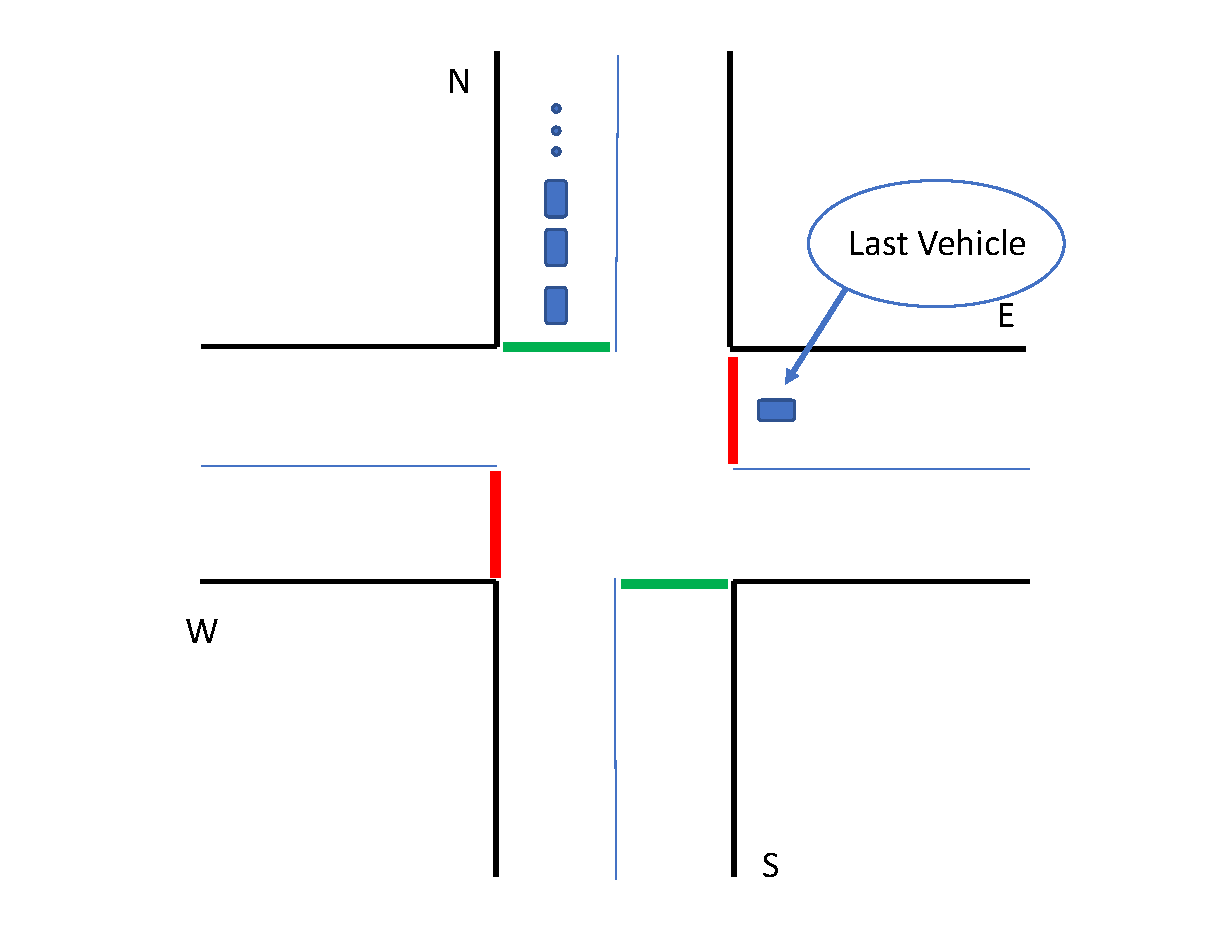
\includegraphics[width=0.9\textwidth]{fig/lastvehicle.pdf}
  \caption{last vehicle}
  \label{fig:last-vehicle}
\end{figure}

\section{改进}
\subsection{目标}
本工作的目的是在提高通行效率(最小化平均通行时间)的同时,希望每条车道能够有尽可能相同的服务延迟(得到放行所需的时间)。这个目标可以用以下的Jain Fairness Index(JFI)指标来量化:
\begin{align}
    \mathcal{J} = \frac{(\sum_{i=1}^{M}\overline{D}_i)^2}{M\sum_{i=1}^{M}\overline{D}_i^2},
\end{align}
其中$\overline{D}_i$是第$i$条进近车道的平均延迟。当且仅当每一个$\overline{D}_i$都相等时,这个指标达到最大值,即是$1$。所以我们的目标也就是最大化这个指标。

\subsection{智能体设计}
\subsection*{状态表示}
在$t$时刻的状态$S(t)$由以下几个部分组成:
\begin{enumerate}
\item 交通流量:$\boldsymbol{V}(t)=\{V_1(t),V_2(t),\cdots,V_M(t)\}$。其中 $V_i(t)$表示第$i$条进近车道上车的数量。值得注意的是,由于右转不受限于信号灯的特殊性,这里我们不考虑右车道的交通流量。
\item 平均吞吐量:$\boldsymbol{\overline{L}}(t)=\{\overline{L}_1(t),\overline{L}_2(t),\cdots,\overline{L}_M(t)\}$。其中$\overline{L}_i(t)$表示第$i$条进近车道的平均吞吐量。同上,不考虑右车道的平均吞吐量。
\item 信号相位:$\boldsymbol{P}(t)$是当前信号相位的数字化表示,$1$表示绿色,可以通行;$0$表示红色,禁止通行。
\end{enumerate}
所以$S(t)=\{\boldsymbol{V}(t) || \boldsymbol{\overline{L}}(t) || \boldsymbol{P}(t) \}$
\subsection*{动作选择}
在本文中,动作选择机制是每次选择即将转换的信号相位。之后,交通信号灯将转换到这一新的相位并持续$\Delta t$的时间。为了安全起见,我们在两个不同的信号相位之间插入了3秒的黄色信号和2秒的红色信号。如果新选择的相位和当前相位相同,则不插入黄色和红色信号,以确保交通流畅。
\subsection*{奖励函数}
受PFS分配原则的启发,我们设计了一个可以在效率和公平之间提供良好的平衡的奖励函数,如下所示:
\begin{align}
\label{eq:reward}
    r = -\sum_{i=1}^{M} \frac{Q_i(t)}{\overline{L}_i(t) + \delta},
\end{align}
其中$Q_i(t)$ 和 $\overline{L}_i(t)$ 分别是第$i$条进近车道的队列长度和平均吞吐量。在每一次调度后(这里,我们将一次动作选择视作一次调度),$\overline{L}_i(t)$ 按照以下方式进行更新:
\begin{align}
    \overline{L}_i(t) = (1-\frac{1}{W})\overline{L}_i(t-1) + \frac{1}{W}L_i(t),
\end{align}
其中$L_i(t)$是此次调度中车道$i$上得到放行的车的数量,$W$是一个平衡通行效率和公平性的参数。另外,为了避免公式\ref{eq:reward}的分母为0, 我们加上了一个可以忽略不计的正数$\delta$。

\begin{figure}[htb]
  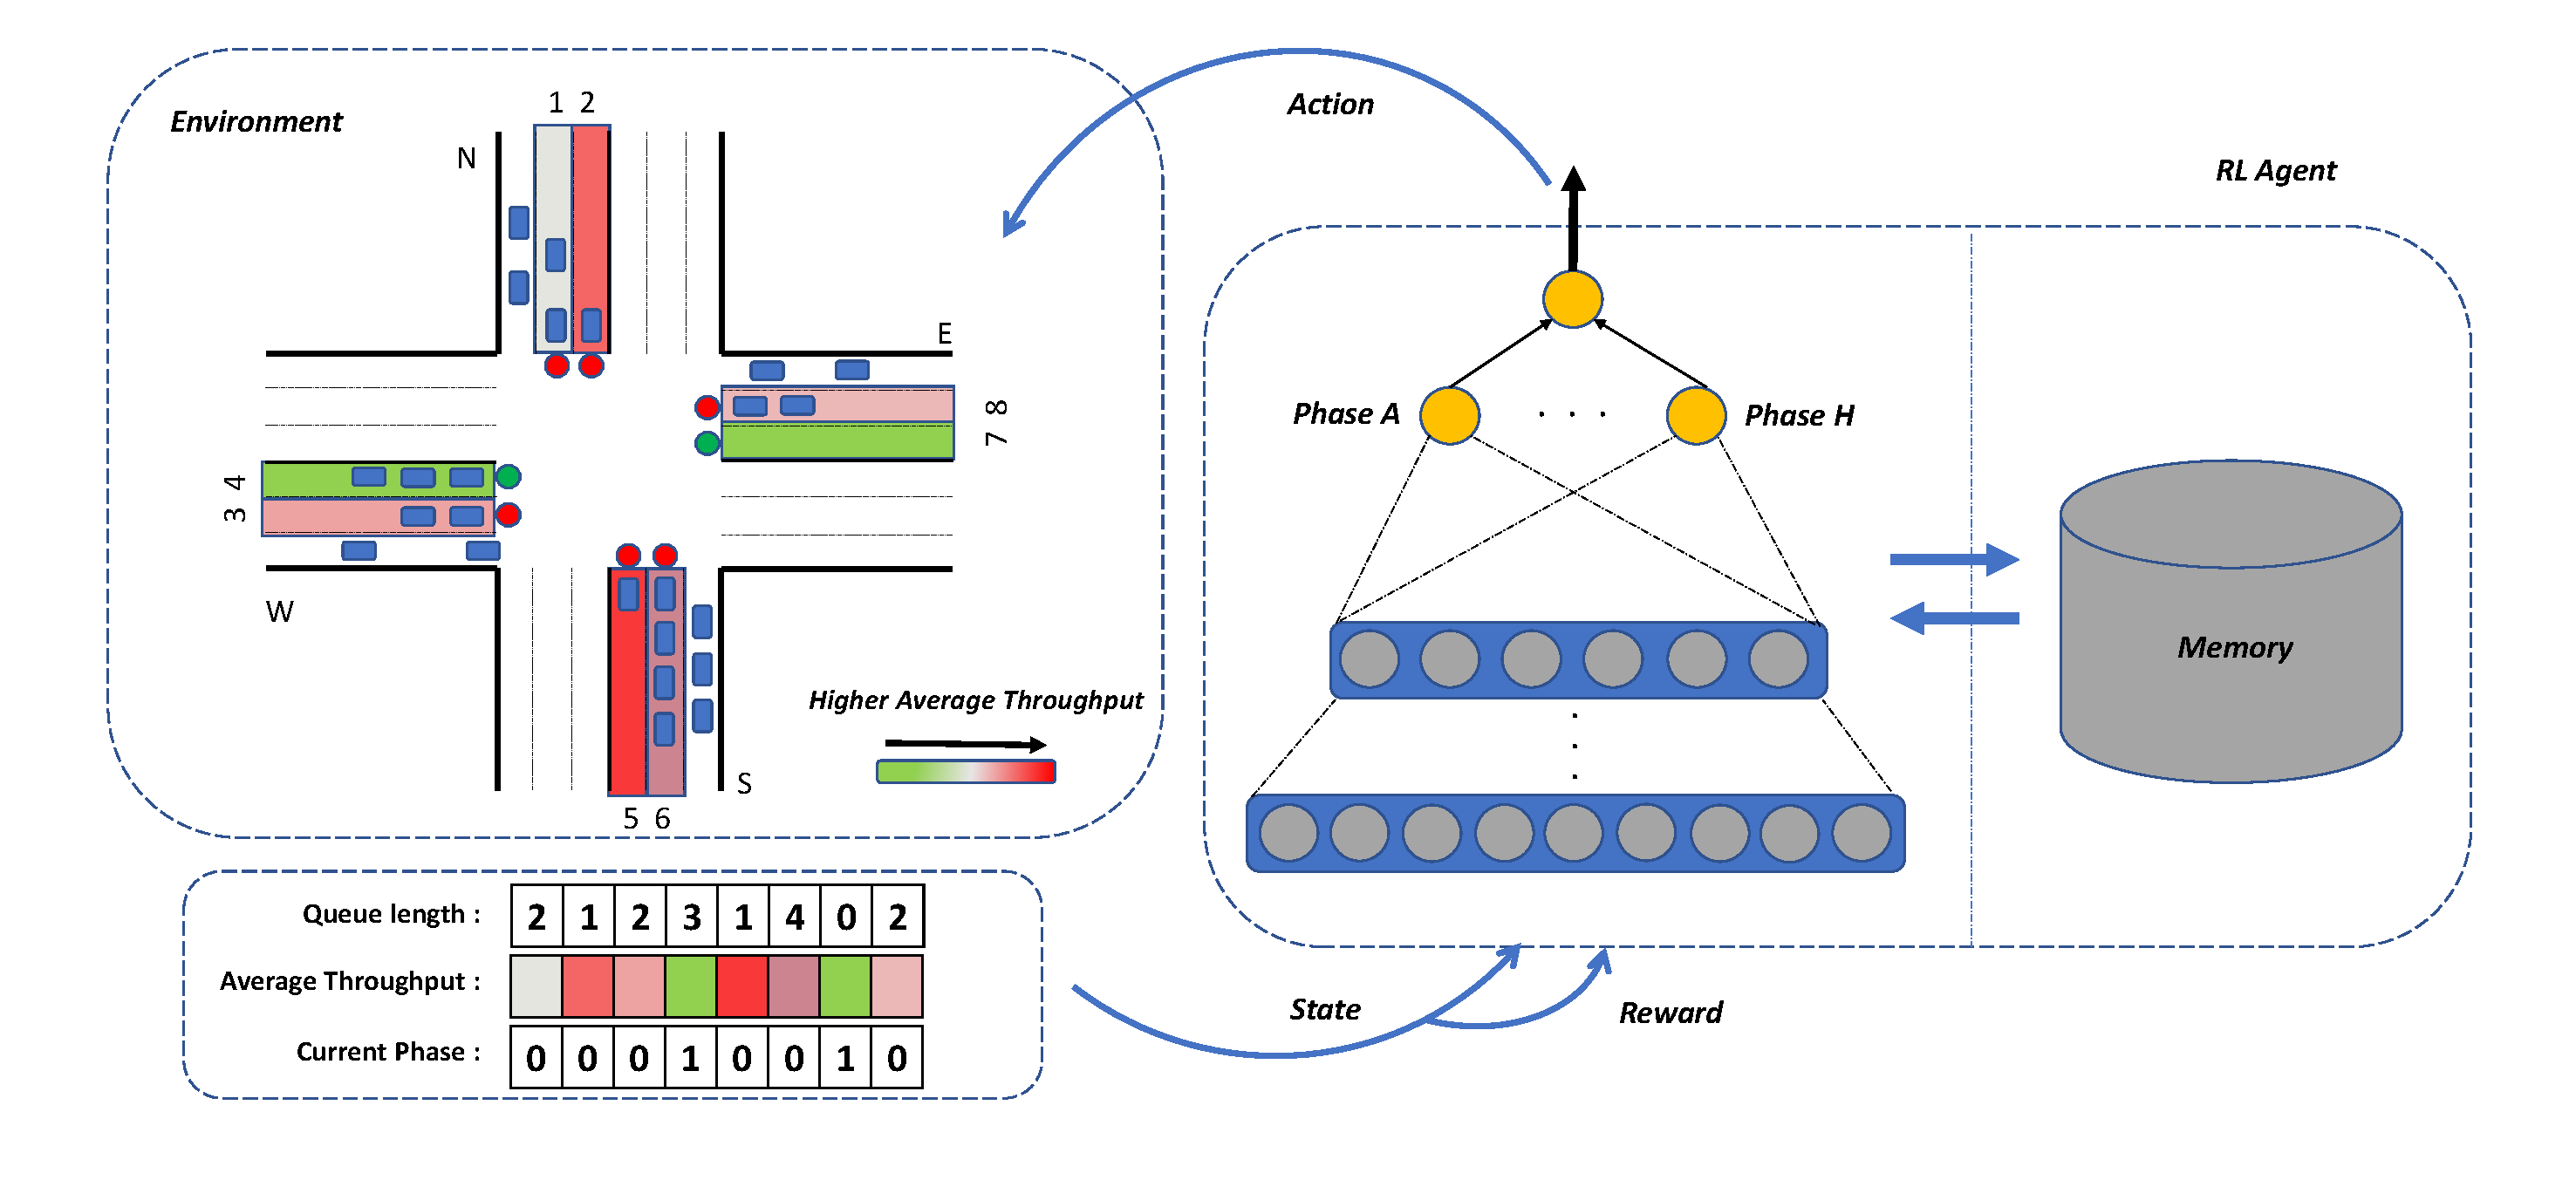
\includegraphics[width=.9\textwidth]{fig/sysmodel.pdf}
  \caption{系统模型}
  \label{fig:system-model}
\end{figure}

\subsection*{训练过程}
如\autoref{fig:system-model}所示,这里我们用DQN作为学习算法,并且采用经验回放\cite{mnih2015human}(experience replay)方法定期提取样本来更新模型,具体算法过程如\autoref{alg:dqn-single}所示。
\begin{breakablealgorithm}
    \caption{基于DQN的交通信号控制训练流程}
    \label{alg:dqn-single}
    \begin{algorithmic}[1] %每行显示行号  
        \Require 
        $E$ : 学习片段数 \newline
        $T$ : 每个学习片段的步数 \newline
        $b$ : 学习经验数 \newline
        $\epsilon$ : 随机选择动作概率 \newline
        $\gamma$ : 折扣因子 \newline
        $\Delta t$ : 信号维持时间
        \For{$episode=1,E$}  
            \State 初始化环境。
            \State 生成车辆。
            \For{$t=1,T$}
                \State 从环境中获取状态观测$s_t$。
                \State 生成一个0到1之间的随机数$rand$。
                \If{ $rand < \epsilon$}
                    \State 从动作空间中随机采样一个动作$a_t$。
                \Else
                    \State 使用DQN模型选择动作:$a_t = \mathop{\arg\max}_a \mathcal{Q}(s_t,a;\theta)$。
                \EndIf
                \State 将当前信号更改为$a_t$并维持$\delta t$秒时间。
                \State 更新每条车道的平均吞吐量。
                \State 环境转移到新的状态$s_{t+1}$并返回一个奖励$r_{t+1}$。
                \State 将经验$(s_t,a_t,r_{t+1},s_{t+1})$ 存储到经验回放池M中。
                \If{$|M|>b$}{
                    \State 从经验回放池M中随机采样b条经验数据。
                    \State 计算损失函数 $\mathcal{L}_j$:
                    $\mathcal{L}_Q=[ r_{t+1}+\gamma \mathop{\arg\max}_{a^{'}} \mathcal{Q}(s_{t+1},a^{'};\theta)-\mathcal{Q}(s_t,a_t;\theta)]^2$;
                    \State 更新DQN参数。
                }
                \EndIf
            \EndFor
        \EndFor  
    \end{algorithmic}  
\end{breakablealgorithm}  

\section{实验}
实验在SUMO(simulation of Urban MObility)\footnote{http://sumo.dlr.de/index.html}仿真平台上进行,利用该模拟器可以方便地实时获取车辆状态,并通过改变交通信号来控制交通运行。我们实现了一个四路交叉口作为我们的实验场景,
交叉口与四个150米长的路段相连,每条道路有三条引入车道和三条引出车道。

我们将N-S方向的道路设置为主干道,车辆到达量更多,将W-E方向的道路设置为次干道,车辆到达量较少。车辆到达服从泊松分布,这里我们设置N-S方向道路的交通流量比率为$\rho$,W-E方向道路的交通流量比率为$1-\rho$,$\rho$值越高,交通流量不平衡的状况越严重。
为了对我们的方法进行综合评价,我们在不同的$\rho$值下进行了实验。注意,为了简化环境,这里我们不考虑行人交通的影响。

\subsection{评价指标}
我们使用以下指标来评估不同方法的效率和公平性表现:
\begin{itemize}
    \item 行驶时间:车辆行驶时间是指车辆进出路口的时间差。现有的大部分工作都集中在最小化所有车辆通过交叉路口的平均行驶时间。
    \item 延误时间:车辆延误时间是车辆通过交叉路口的实际时间与预期时间(以最高限速通过交叉路口所需的时间)之间的差值。
    \item 驾驶体验得分:此外,我们提出了一种新的评价指标,称为驾驶体验得分(Driving Experience Score,DES),来量化驾驶员的满意度,具体评分标准见下表:
        \begin{table}[htb]
            \caption{驾驶体验得分标准}
            \begin{tabular}{cc}
            \toprule
            延误时间(s) & DES \\
            \midrule
            $d \leq 40$ & 5\\
            $40 < d \leq 80$ & 4 \\
            $80 < d \leq 120$ & 3 \\
            $120 < d \leq 160$ & 2 \\
            $d > 160$ & 1 \\ 
            \bottomrule
            \end{tabular}
        \end{table}
        事实上,可能有更多的因素需要考虑(如燃油消耗),但是这里的目的是为了缓解车辆的过度延误情况,因此我们这里用延误时间作为评价标准。
\end{itemize}
\subsection{比较方法}
\begin{itemize}
    \item FT(Fixed-Time Control\cite{miller1963settings}):这种方法以预先设定的方式循环改变信号。
    \item SOTL(Self-Organizing Traffic Light Control\cite{cools2013self}):这是一种根据预先设定的阈值来改变信号的自适应方法。如果等待的车辆数量超过了这个阈值,则切换到下一个信号相位。
    \item LIT\cite{zheng2019diagnosing}:这是一种基于学习的方法,比大多数现有的致力于提高通行效率的方法效果更好。
    \item FIT(\textbf{F}airness-aware \textbf{I}ntelligent \textbf{T}raffic Light Control):我们的方法。
\end{itemize}
\subsection{性能评价}
首先,我们通过实验评估了不同方法的通信效率的表现,为了得到一个综合的结果,我们在不同的$\rho$值下进行了实验,实验结果如\autoref{fig:efficiency}所示。
可以观察到,我们的方法(FIT)的车辆通过路口的平均行驶时间远低于传统方法(行驶时间越短意味着效率越高),并且仅略低于只注重效率的LIT方法。
\begin{figure}[htb]
    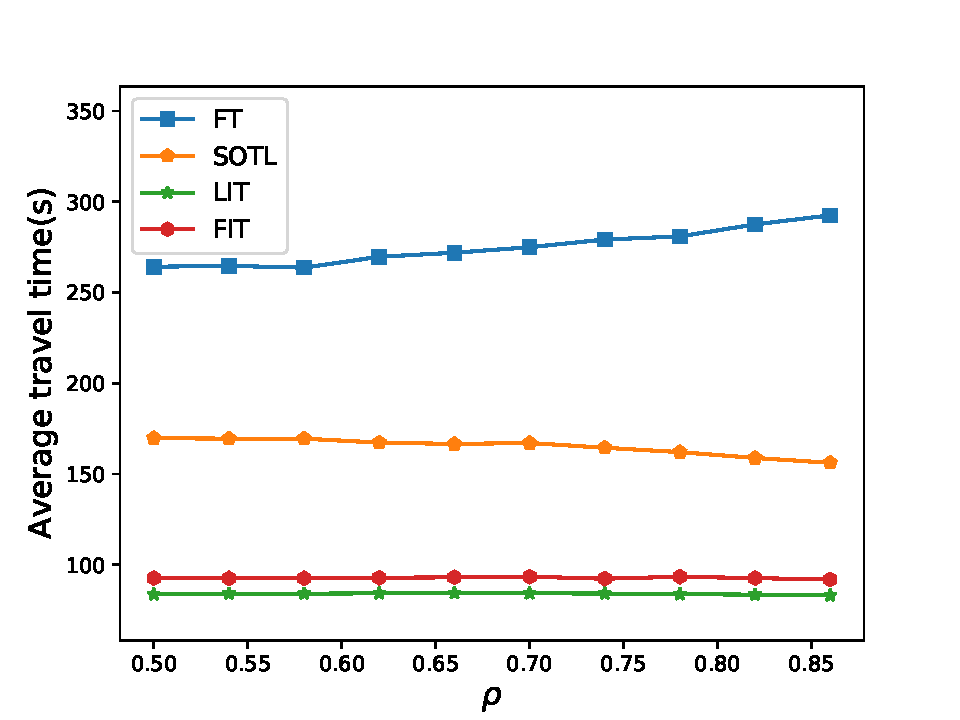
\includegraphics[width=10cm]{fig/efficiency.pdf}
    \caption{效率}
    \label{fig:efficiency}
\end{figure}

其次,由于我们的主要研究目标是公平性,我们首先分析了在使用不同方法下每条车道的延误情况。这里我们用Jain Fairness Index(JFI)来量化公平性指标,JFI的计算方式如下:
\begin{align}
    \mathcal{J}=\frac{\left(\sum_{i=1}^{M} \bar{D}_{i}\right)^{2}}{M \sum_{i=1}^{M} \bar{D}_{i}^{2}},
\end{align}
其中$\bar{D}_{i}$是车道$i$的平均延误时间。当每个车道具有相同的平均延误时间时,JFI的值达到最大值,即1。\autoref{fig:fairness}展示了四种方法在不同$\rho$值下的平均延迟的JFI表现。从中我们可以看出FT和LIT的JFI值随着交通不平衡情况的加剧(即$\rho$值越大)而减小,而FIT任然能偶保持较高的值,并且高于同样能够保持稳定JFI值的SOTL方法。
\begin{figure}[htb]
    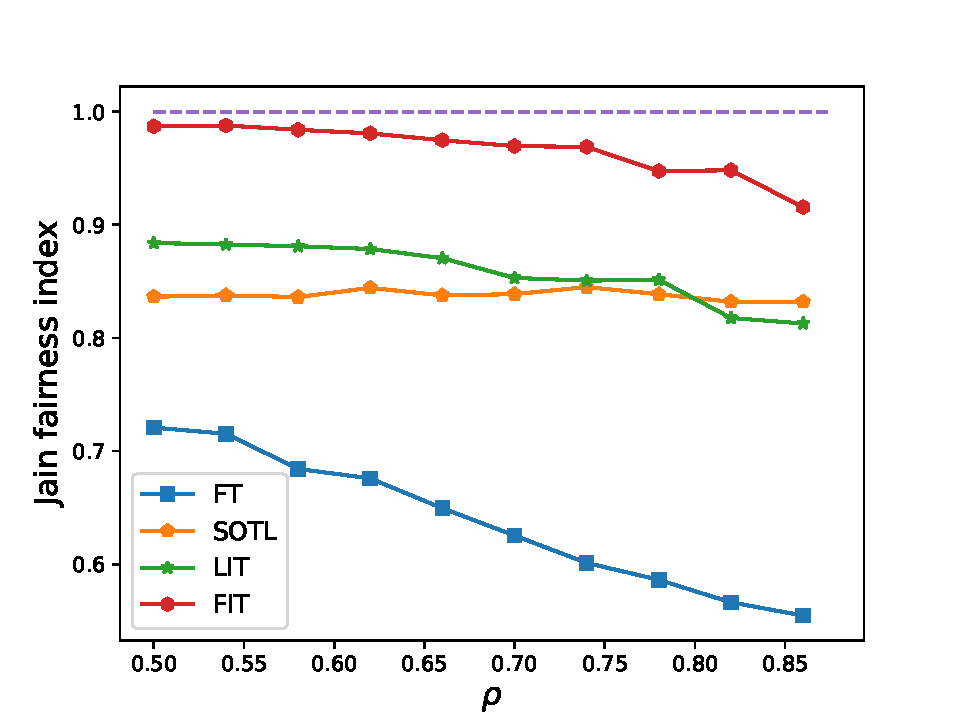
\includegraphics[width=10cm]{fig/fairness.pdf}
    \caption{公平}
    \label{fig:fairness}
\end{figure}

然后,我们更加详细地研究了不同方法的延误情况。下面我们具体分析在主干道和支干道上四种方法在不同的$\rho$值情况下车辆延误时间分布情况。
\begin{figure}[htb]
    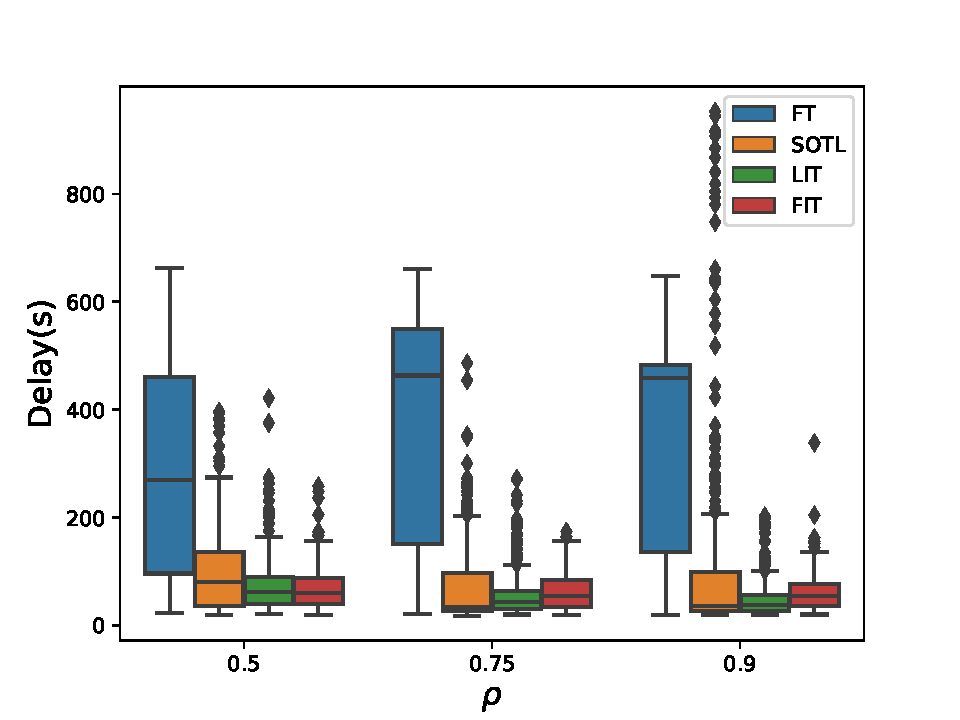
\includegraphics[width=10cm]{fig/major_delay.pdf}
    \caption{主干道(N-S方向)的车辆延误时间分布}
    \label{fig:major_delay}
\end{figure}
从\autoref{fig:major_delay}中我们可以看出,在主干道上,基于学习的方法(LIT和FIT)比传统方法(FT和SOTL)具有更低的延误时间,虽然SOTL方法整体上延迟也比较低,但是会有很多极端值,最高的延误时间甚至超过800$s$。

从\autoref{fig:minor_delay}中我们可以看出,在支干道上,随着$\rho$值的增加(即交通不平衡情况的加重),原先在主干道上表现优异的LIT方法性能开始恶化(),但是FIT依然能够保持一个相对低的延迟。

\begin{figure}[htb]
    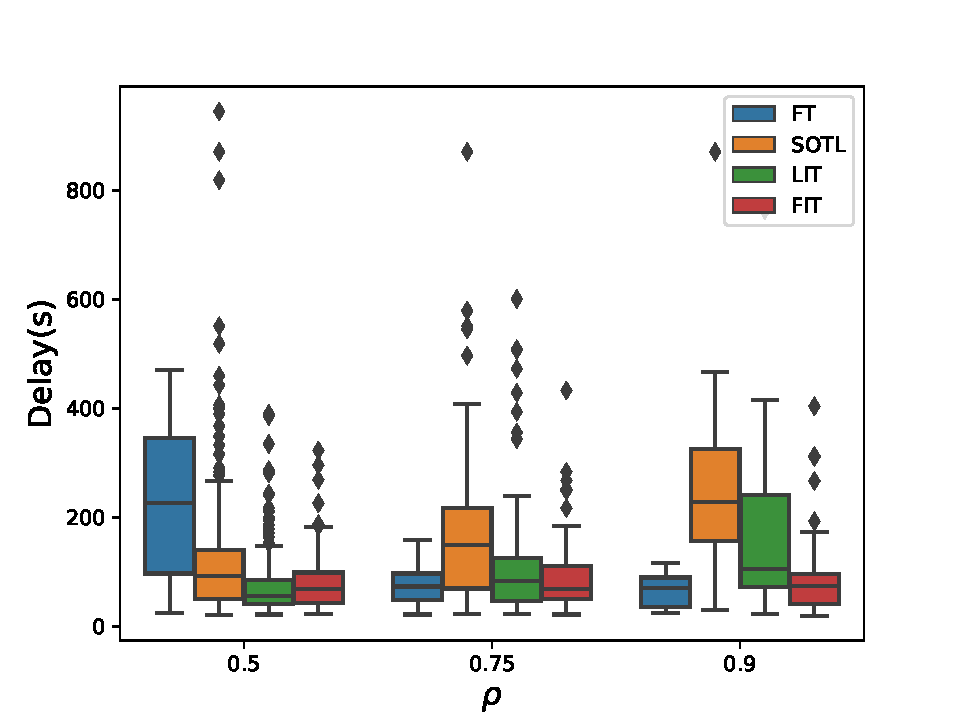
\includegraphics[width=10cm]{fig/minor_delay.pdf}
    \caption{支干道(N-S方向)的车辆延误时间分布}
    \label{fig:minor_delay}
\end{figure}

我们研究了不同方法的驾驶体验得分情况,\autoref{fig:des}展示了在$\rho=0.75$的情况下不同方法的驾驶体验得分分布情况。从中我们可以看出,FT方法超过半数的驾驶体验的分都是1分,由此可以看出该方法的不灵活。对于SOTL方法而言,虽然他的5分的比例最高,但是其得分分布的方差也是最高的。FIT的得分分布与LIT相似,但FIT的方差低于LIT,在以牺牲少量效率为代价的前提下。
\begin{figure}[t]
    \centering
    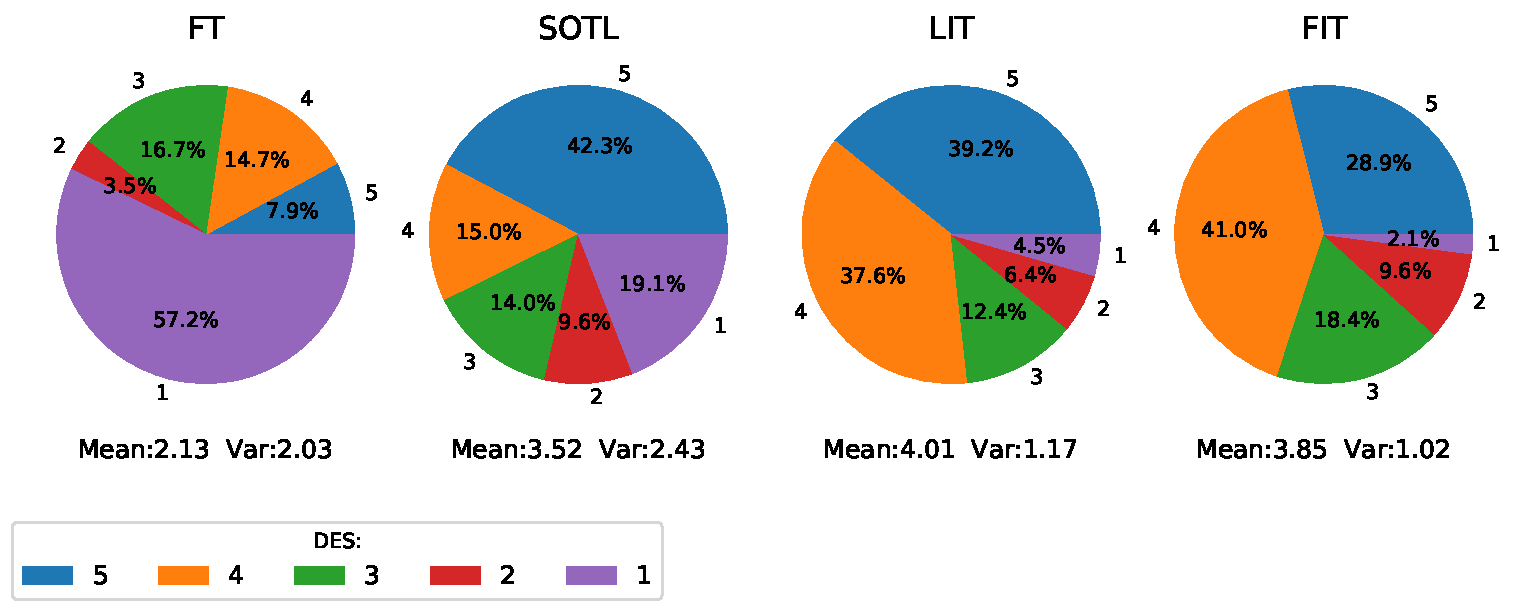
\includegraphics[width=0.9\textwidth]{fig/des.pdf}
    \caption{驾驶体验得分统计}
    \label{fig:des}
\end{figure}

最后,我们研究了$W$参数的影响,因为$W$是用来平衡效率和公平性的,不同的值会导致学习到不同的策略,从\autoref{fig:window-size}中我们可以看出W值越高,越有利于系统的公平性。相反,W值越小,系统效率就越高。具体来说,当$W=1$时,我们方法FIT的整体性能接近于LIT
\begin{figure}[htb]
    
    \subfloat[效率\label{fig:window-size-efficiency}]{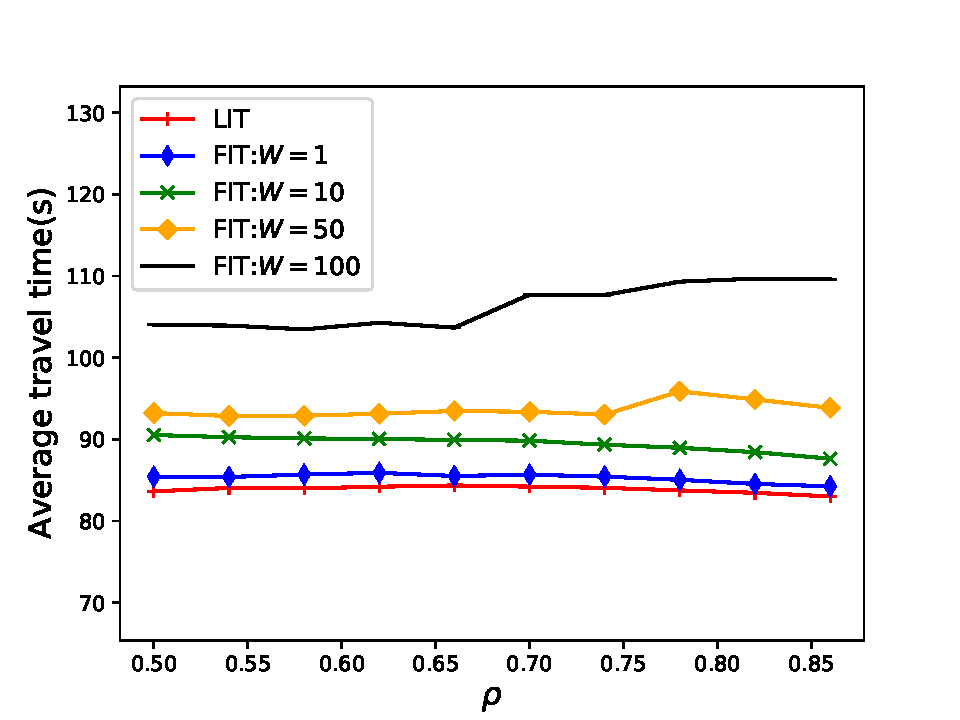
\includegraphics[width=0.4\textwidth]{fig/window_efficiency.pdf}}
    \subfloat[公平性\label{fig:window-size-fairness}]{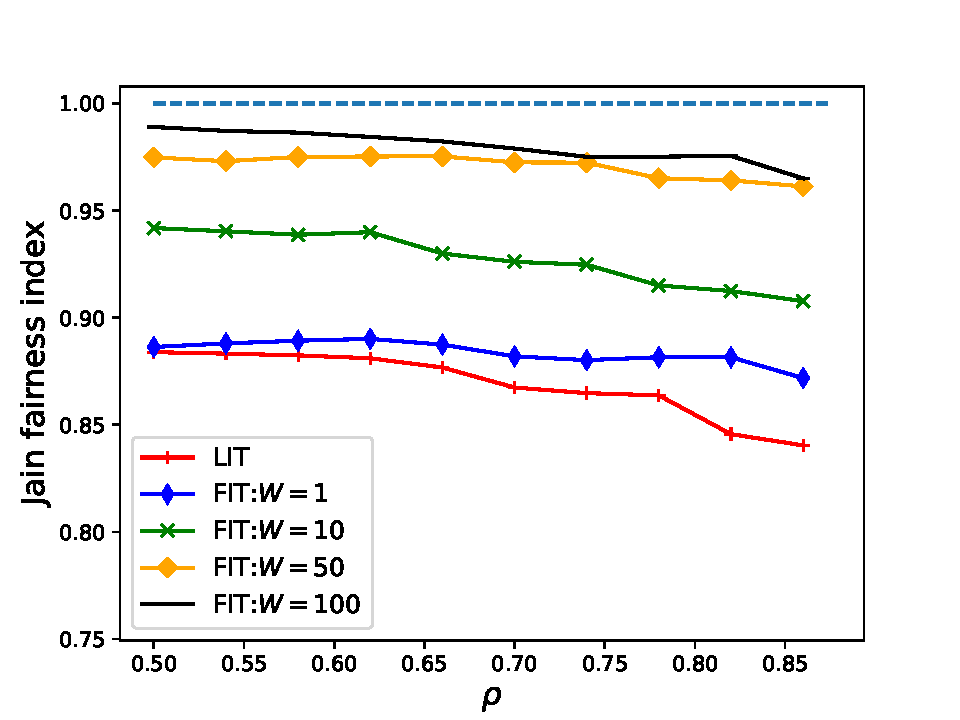
\includegraphics[width=0.4\textwidth]{fig/window_fairness.pdf}}
    \caption{$W$对效率和公平性的影响}
    \label{fig:window-size}
  \end{figure}




\chapter{多路口场景智能交通信号调度}

\section{相关工作}
由于强化学习在单路口交通信号控制上取得了优异的成绩,人们开始致力于使用多智能体强化学习(Multi-Agent Reinforcement Learning, MARL)来解决多路口场景下的交通信号调度。Claus在\inlinecite{claus1998dynamics}中将MARL分为了两类:联合动作学习(Joint Action Learning)和独立学习(Independent Learning)。

对于多路口信号控制,联合动作学习的思想就是使用一个全局智能体(single global agent)来控制所有的交叉路口,其动作是所有路口动作组合在一起的联合动作,然后通过迭代学习建模多个智能体的联合动作价值函数(Joint Action Value Function):
\begin{align}
  Q(o_1, o_2, \cdots, o_N, \mathbf{a})
\end{align}
其中$o_i$是智能体$i$对路口环境的观测,$\mathbf{a}$是所有智能体的联合动作。但是这种方法的缺点是会导致维度灾难(curse of dimensionality),状态动作的联合空间会随着智能体数量的增加呈指数级增长,增加学习的难度。为了缓解这个问题,\inlinecite{van2016coordinated}使用max-plus方法将联合动作价值函数分解为局部子问题的线性组合,如下所示:
\begin{align}
  \hat{Q}\left(o_{1}, \ldots, o_{N}, \mathbf{a}\right)=\Sigma_{i, j} Q_{i, j}\left(o_{i}, o_{j}, \mathbf{a}_{i}, \mathbf{a}_{j}\right)
\end{align}
其中$i \text{和} j$对应于相邻智能体的索引。在\inlinecite{zhang2019integrating,chu2019multi,tan2019cooperative}中,将联合Q值视为局部Q值的加权和:
\begin{align}
  \hat{Q}\left(o_{1}, \ldots, o_{N}, \mathbf{a}\right)=\Sigma_{i, j} w_{i, j} Q_{i, j}\left(o_{i}, o_{j}, \mathbf{a}_{i}, \mathbf{a}_{j}\right)
\end{align}
其中$w_{i,j}$是预先定义的权重。他们试图通过在单个智能体的学习过程的损失函数中增加一个整形项,并使单个Q值的加权和与全局Q值的差异最小化,从而确保单个智能体在学习过程中能够考虑到其他智能体的情况。

多路口信号控制的另一条研究路线是使用独立的RL(IRL)智能体来控制交通信号,其中每个RL智能体控制一个路口。与联合动作学习方法不同,每个智能体可以在不知道其他智能体的奖励信号的情况下学习控制策略。根据智能体之间是否进行信息交互进一步分为以下两类:
\begin{itemize}
  \item IRL without Communication:IRL单独处理每个交叉口,每个agent观察自己的本地环境,不使用显式通信来解决冲突\inlinecite{mannion2016experimental,casas2017deep,zheng2020learning,pham2013learning,liu2018deep,calvo2018heterogeneous,gong2019decentralized}。在一些简单的场景中,如动脉网络,这种方法表现良好,可以形成了几个小绿波(Green waves)。
  然而,当环境变得复杂时,来自相邻agent的非平稳影响将被带到环境中,如果agent之间没有通信或协调机制,学习过程通常无法收敛到平稳策略。为了应对这一挑战,wei在\inlinecite{wei2019presslight}中提出了一个特定的奖励函数,去描述相邻智能体之间的需求从而实现协调。
  
  \item IRL with Communication:这种方法使智能体之间能够就他们的观察进行交流,并作为一个群体而不是个体的集合来完成复杂的任务,在这种情况下,环境是动态的,每个智能体的能力和对世界的可见度是有限的\inlinecite{sukhbaatar2016learning}。
  典型的方法是直接将邻居的交通状况\inlinecite{xu2020network}或过去的动作\inlinecite{ge2019cooperative}加入到自身智能体的观察中,而不是仅仅使用自我观测到的本地交通状况。在这种方法中,不同路口的所有智能体共享一个学习模型,这就需要对相邻的路口进行一致的索引。
  \inlinecite{nishi2018traffic}试图通过利用图卷积网络的路网结构来消除这一要求,以协作附件的多跳路口的交通,并且通过图卷积网络中定义的固定邻接矩阵来模拟相邻代智能体的影响,这表明他们假设相邻智能体之间的影响是静态的。
  在其他工作中,\inlinecite{wei2019colight,wang2020stmarl}提出使用图注意网络来学习相邻智能体和自我智能体的隐藏状态之间的动态相互作用。应该指出的是,利用max-plus学习联合行动学习者的方法和利用图卷积网络学习通信的方法之间有很强的联系,因为它们都可以被看作是学习图上的信息传递,其中前一种方法传递奖励,后一种方法传递状态观测信息。
\end{itemize}

\section{已有工作中的不足}
目前大多数工作在使用图神经网络Learn to Communicate的时候,都是以intersection为节点来进行图建模,将每一个路口视作图中的一个节点,每条道路作为连接两个节点的边,很自然地可以将一张交通道路网建模成一个图, 如\autoref{fig:network-graph-old}所示:
\begin{figure}[htb]
  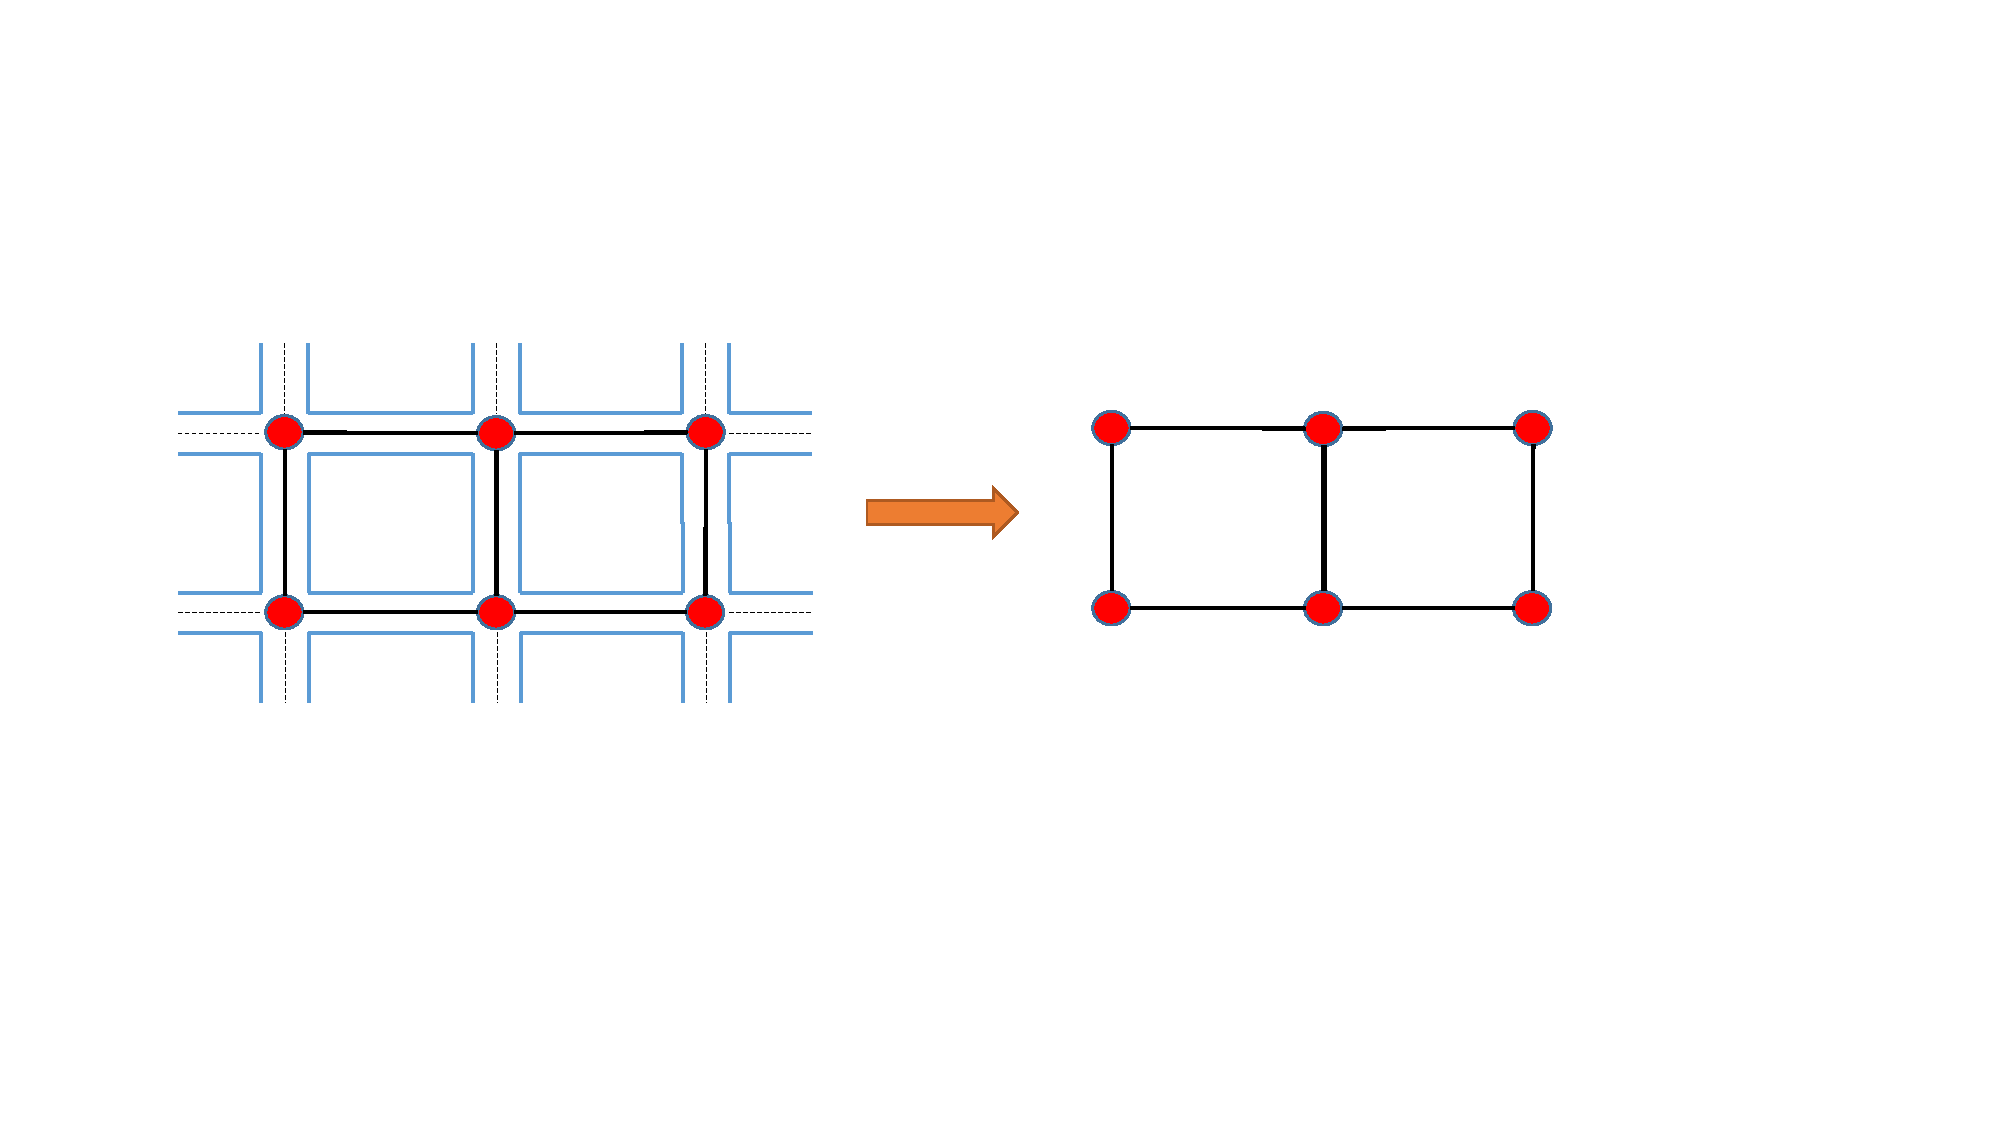
\includegraphics[width=1.2\textwidth]{ppt/network-graph.pdf}
  \caption{以路口为节点的建图方式示意图}
  \label{fig:network-graph-old}
\end{figure}
在这种建模方式下,每条车道的车辆以及当前的相位将作为该节点的特征。这种建模方式虽然可以很清晰的将多路口场景变成一张图。但是,因为是以一个路口为一个节点,所有车道的状态信息都整合到了一起,有些车道的的信息对目标节点是无用的,
如\autoref{fig:information-redundancy}所示:
\begin{figure}[htb]
  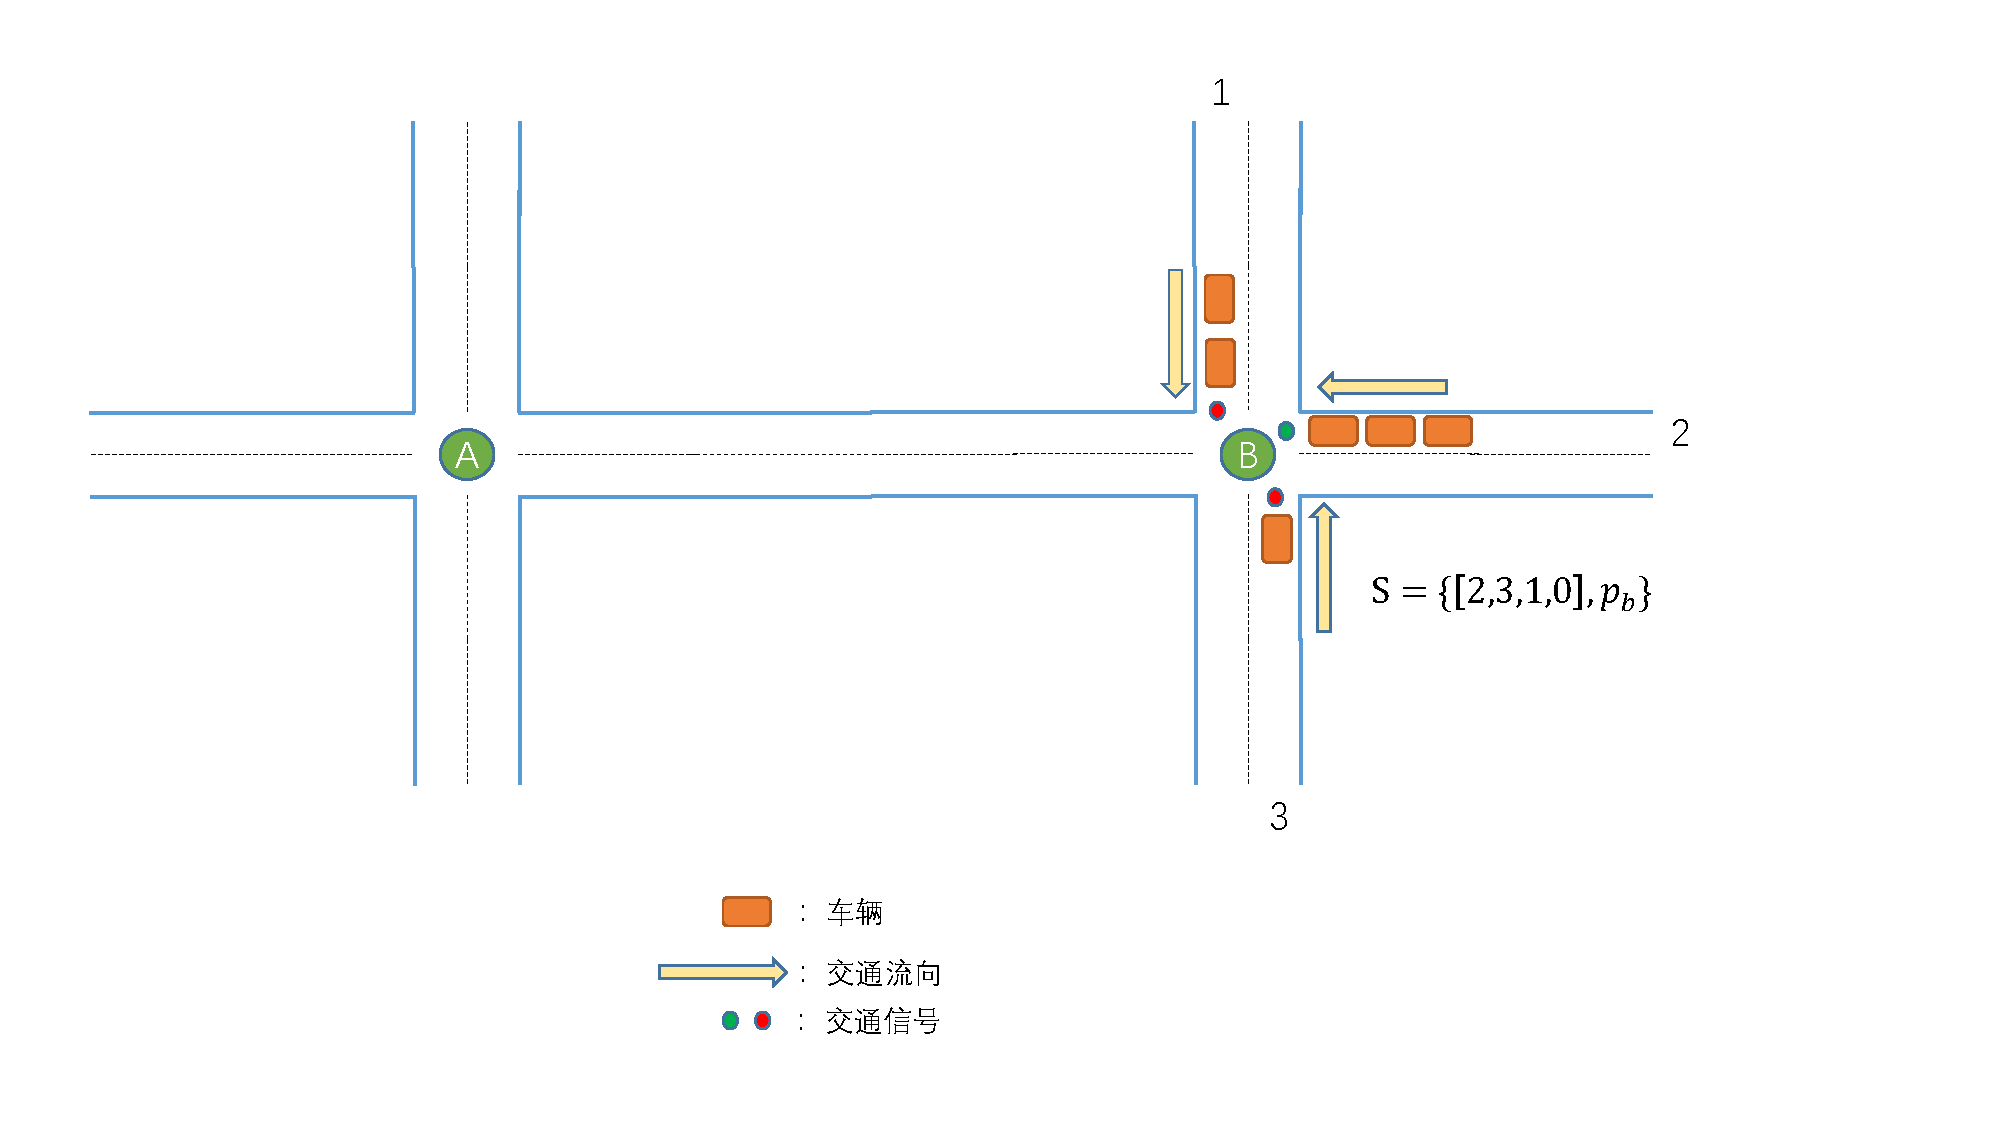
\includegraphics[width=1.2\textwidth]{ppt/information-redundancy.pdf}
  \caption{在以路口为节点的建图方式下的信息传递示意图}
  \label{fig:information-redundancy}
\end{figure}
路口B中只有车道2的交通流向与路口A有关,车道1和车道3的车辆不会行驶到路口A。在信息传递的时候,如果将路口B所有的信息都笼统地传递过去,将会增加路口A的智能体提取有效信息的难度,从而降低学习的效率。

\section{改进}
\subsection{目标}
我们的目标是在进行信息交互的时候能够剔除与目标节点无关的信息,从而降低目标节点聚合邻居节点信息的难度,提高学习效率。

\subsection{基于道路的图建模方式}
本文同样采用IRL with Communication的框架,与已有工作不同的是,我们采用不同的建模方式:以道路为节点进行图建模,即一条道路就是一个节点,如\autoref{fig:network-graph-new}所示:
\begin{figure}[htb]
  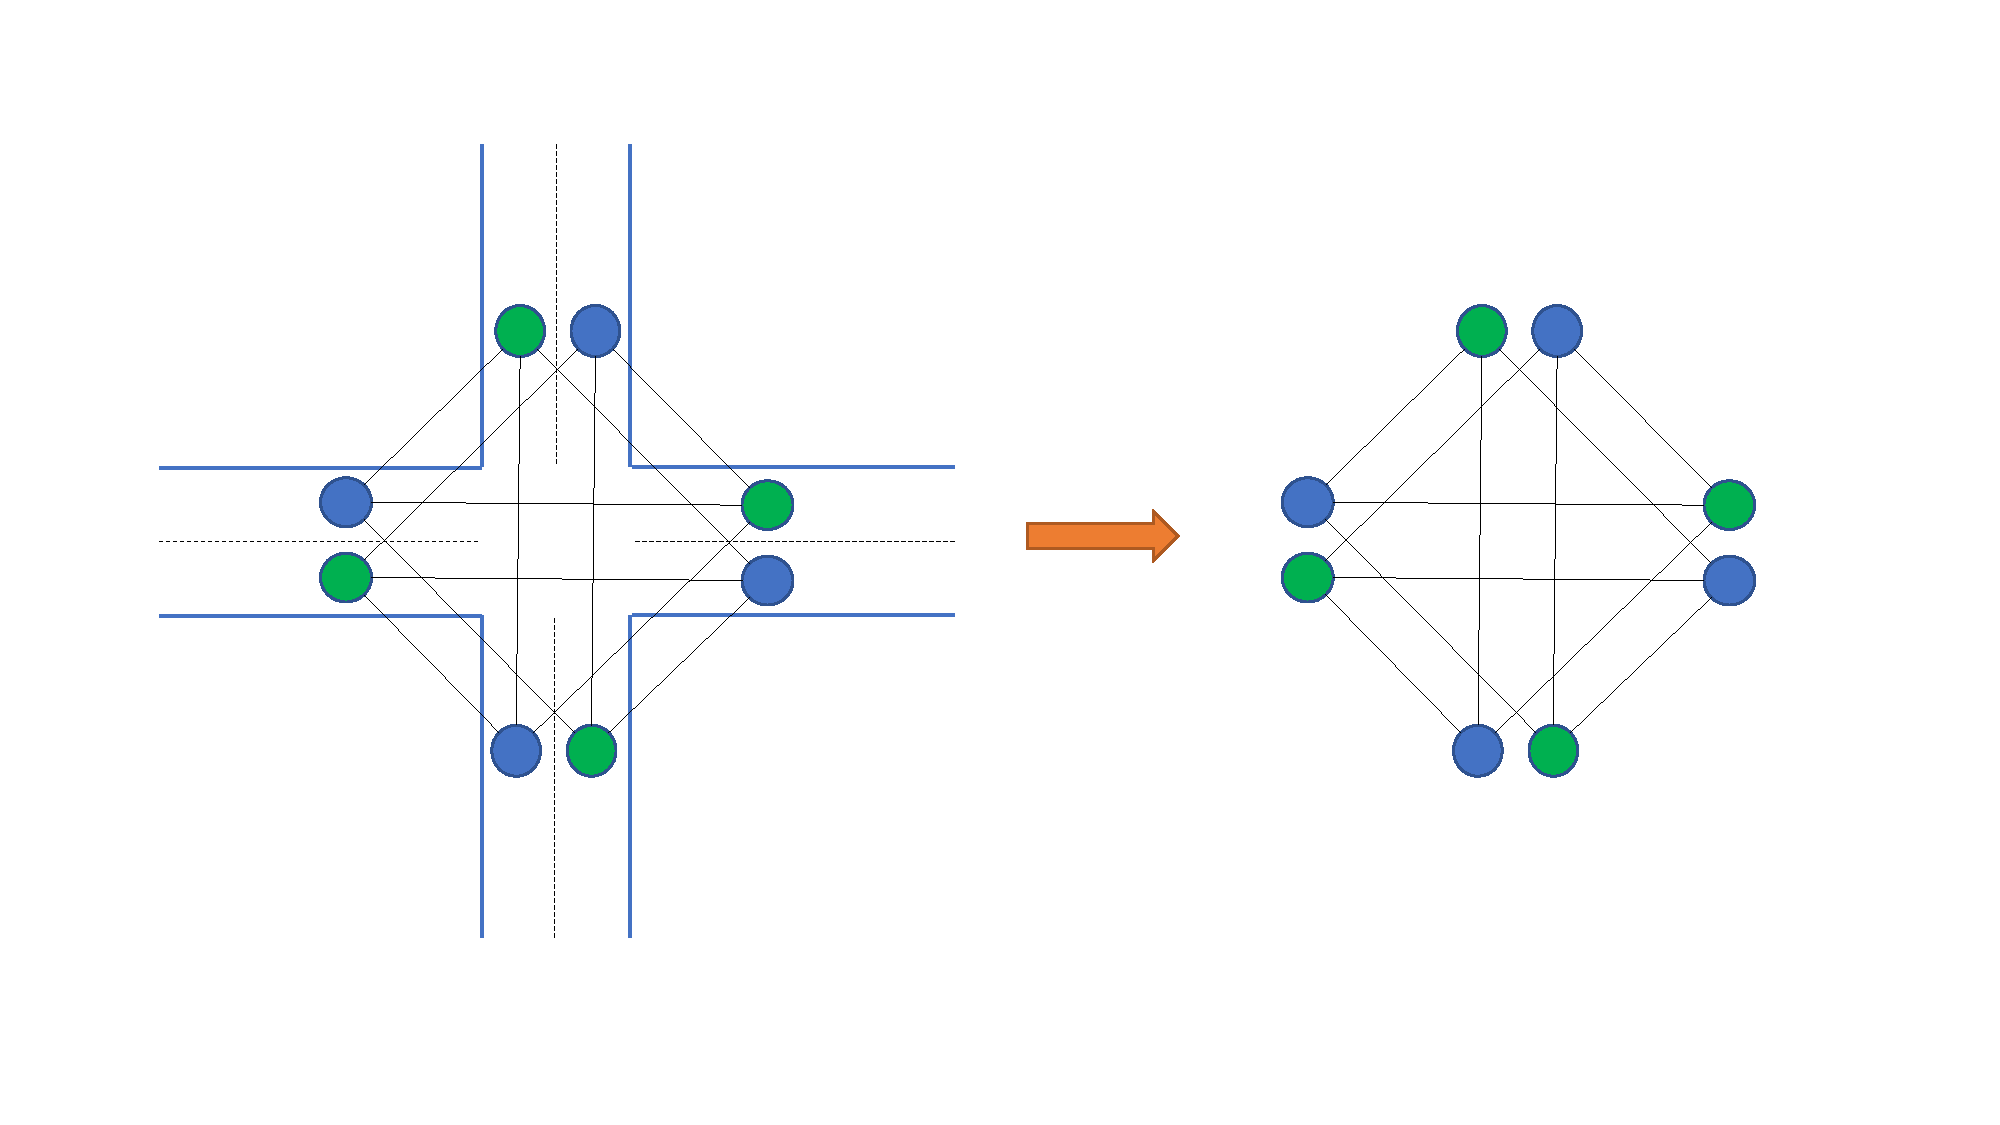
\includegraphics[width=0.9\textwidth]{ppt/graph-modeling.pdf}
  \caption{以道路为节点的建图方式示意图}
  \label{fig:network-graph-new}
\end{figure}

此外,我们根据当前的信号相位对图的边设一个权重。这里我们规定,如果在当前相位下,道路$i$到道路$j$之间的交通是允许通行的,则表示$(i,j)$的状态是'connected',权重的具体定义方法如下:
\begin{align}
  w_{i,j} = \begin{cases}
    1 & (i, j) \text{ is connected} \\
    0 & \text{otherwise}
  \end{cases}
\end{align}
这个权重$w_{i,j}$将被用于剔除对目标节点无用的信息。

\subsection{Learn to Communicate}
这里我们沿用\inlinecite{wei2019colight,wang2020stmarl}工作使用图注意网络,但是与之不同的是,我们不是用来学习目标节点和邻近节点的隐藏状态之间的动态相互作用,而是用来做节点回归(Node Regression),即估计目标节点在下一个时间点的特征。具体包括以下几个过程:
\begin{itemize}
  \item 重要性计算:为了了解节点$j$(源节点)的信息在确定节点$i$(目标节点)下一时刻的特征的重要性,我们首先嵌入两个节点的特征,然后计算他们之间的相关系数$e_{i j}$(节点$j$在确定节点$i$的特征时的重要性),具体操作如下:
  \begin{align}
    e_{i j}=a\left(\left[W h_{i} \| W h_{j}\right]\right)
  \end{align}
  其中$W$是一个共享参数,用来进行特征增强,然后用$[\cdot \| \cdot]$对节点$i$和节点$j$增强后的特征进行拼接,最后使用$a(\cdot)$将拼接后的高维特征映射到一个实数上。
  
  \item 特征筛选:由于当前交通信号的影响,道路$j$的车辆不会进入到道路$i$,即节点$j$的信息在确定节点$i$的下一时刻的特征时是无用的,因此我们要筛选掉对目标节点无用的信息。这里我们通过之前介绍的边的权重来实现:
  \begin{align}
    \label{eq:mul_phase}
    e_{i j} = e_{i j} * w_{i,j},
  \end{align}
  如果$WE_{i j} = 1$(即道路$j$到道路$i$的交通在当前相位下是可以通行的),$e_{ij}$将维持之前的计算结果。反之,如果$w_{i,j}=0$,将清除节点$j$对节点$i$的影响。
  
  \item 注意力分布计算:为了重新确定源节点和目标节点之间的注意力值,我们进一步将目标节点$i$和其邻近节点之间的交互等分进行归一化:
  \begin{align}
    \alpha_{i j}=\operatorname{softmax}\left(e_{i j}\right)=\frac{\exp \left(e_{i j} / \tau\right)}{\sum_{j \in \mathcal{N}_{i}} \exp \left(e_{i j} / \tau\right)},
  \end{align}
  其中$\tau$是一个温度系数,$\mathcal{N}_{i}$是目标节点$i$邻近范围的节点集合。
  \item 特征回归:为了确定目标节点在下一个时刻的特征,这里我们将其所有邻近节点的信息按照各自的重要性进行组合:
  \begin{align}
    h_{i}^{\prime}=\sigma\left(\sum_{j \in \mathcal{N}_{i}} \alpha_{i j} W h_{j}\right)
  \end{align}
  其中$\sigma(\cdot)$是激活函数。$h_{i}$是$i$节点融合了邻域信息后的新特征。
  \item Multi-Head Attention:进一步,我们使用多头注意力机制(Multi-Head Attention)来关注不同相关性下的信息,如下所示:
  \begin{align}
    h_{i}^{\prime}(K)=\sigma\left( \frac{1}{K} \sum_{k=1}^{k=K} \sum_{j \in \mathcal{N}_{i}} \alpha_{i j}^{k} W^{k} h_{j}\right)
  \end{align}
  其中$K$是注意力头的数量,例如当$k = 3$时,结构如图\autoref{fig:multi-head}所示:
  \begin{figure}[htb]
    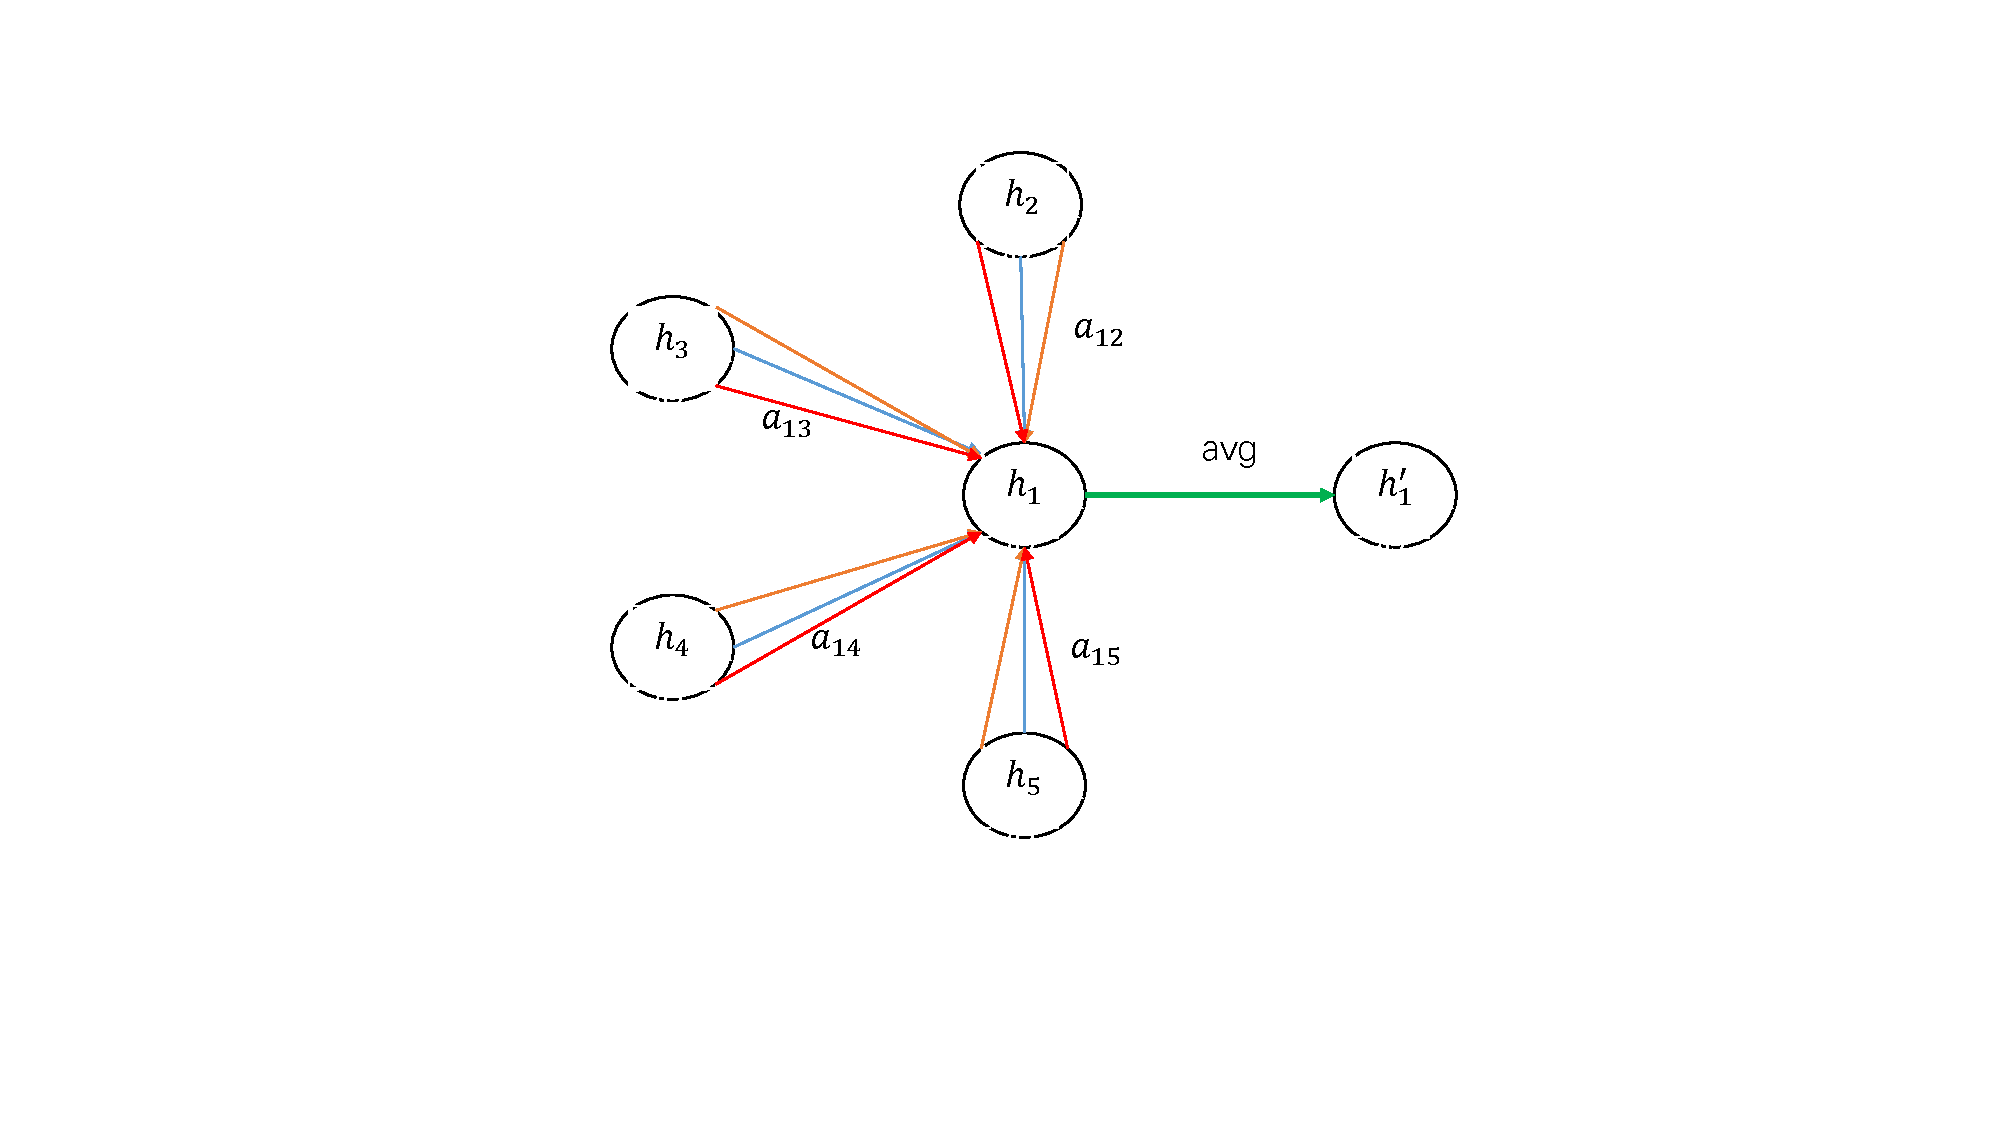
\includegraphics[width=0.9\textwidth]{fig/multi-head.pdf}
    \caption{多头注意力计算示意图($k=3$)}
    \label{fig:multi-head}
  \end{figure}
\end{itemize}

对于每个路口,我们要估计每条引进道路在下一调度时刻的状态,即我们要对四个节点进行计算,如\autoref{fig:node-regression}中A路口的四个红色节点。通过在目标节点(红色节点)的及其邻近节点(绿色节点)构成的子图(如图\autoref{fig:node-regression}中右上角的图)上对目标节点进行上述的计算。
\begin{figure}[htb]
  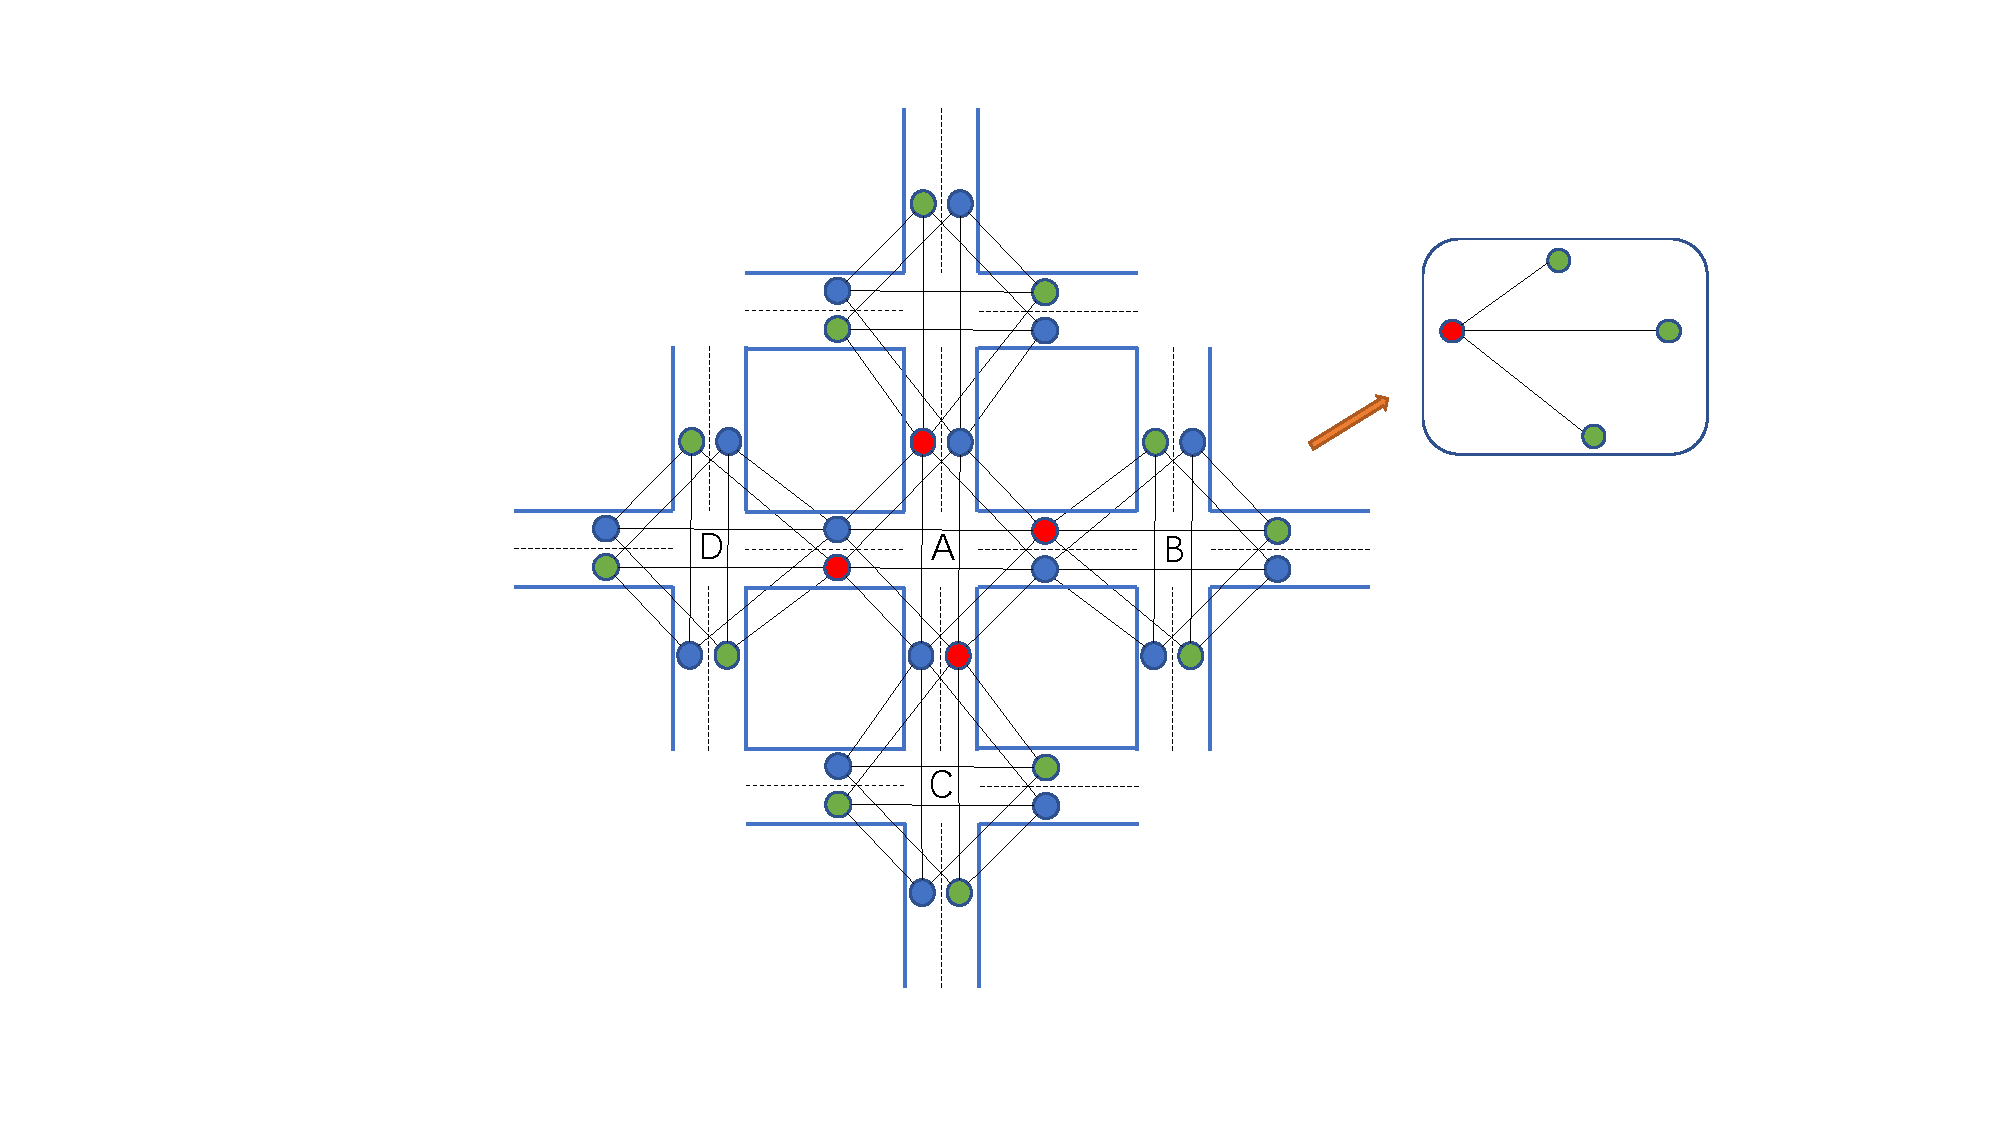
\includegraphics[width=0.9\textwidth]{fig/node-regression.pdf}
  \caption{节点回归计算示意图}
  \label{fig:node-regression}
\end{figure}
由于我们是以道路为节点进行建图的,所以即便是单个路口也可以表示成一个图,所以当有多个路口的时候,会产生一张很大的图。这里每个节点维护自己路口的子图,包括更新子图中的节点特征以及边的权重(根据当前路口的信号相位确定)。

\subsection{模型框架}
如\autoref{fig:model-framework}所示,对于单个路口来说,有两个模型,一个是用来进行交通信号控制的DQN模型$\mathcal{Q}$,另一个是用来预测下一调度时刻状态的GAT模型$\mathcal{G}$。
对于DQN模型来说,每次根据输入的状态来选择动作,其中状态由以下几部分组成:
\begin{itemize}
  \item Queue length:当前路口每条车道的队列长度。
  \item Traffic volume:当前路口每条车道的车辆数。
  \item Current Phase:路口当前的相位。
  \item Next Queue length:通过节点回归估计的下一调度时刻的Queue length。
  \item Next Traffic Volume:通过节点回归估计的下一调度时刻的Volume。
\end{itemize}
其损失函数如\autoref{eq:loss-dqn}所示:
\begin{align}
  \label{eq:loss-dqn}
  \mathcal{L}_t=[ r_{t+1}+\gamma \mathop{\arg\max}_{a^{\prime}} \mathcal{Q}(s_{t+1},a^{'};\theta)-\mathcal{Q}(s_t,a_j;\theta)]^2,
\end{align}

对于GAT模型来说,首先我们规定节点的特征$f_t=\{q_t, v_t\}$,其中$q_t$和$v_t$分别时队列长度(Queue length)和交通流量(Traffic volume)。当环境转移到新的状态$s_{t+1}$时,更新节点特征($f_{t+1}=\{q_{t+1},v_{t+1}\}$)以及边的权重,其损失函数如下所示:
\begin{align}
  \label{eq:loss-gat}
  \mathcal{L}_G = [f_{t+1} - f_{t+1}^{\prime}]^2
\end{align}
其中$f_{t+1}^{\prime}$是在$t$调度时刻,利用邻近节点信息预估的下一时刻的节点特征,是预测值,而$f_{t+1}$是$t+1$时刻的真实节点特征。

具体的算法流程如\autoref{alg:dqn-gat}所示。
\begin{breakablealgorithm}
  \caption{multi-intersection}
  \label{alg:dqn-gat}
  \begin{algorithmic}[1] %每行显示行号  
      \Require 
      $E$ : 学习片段数 \newline
      $T$ : 每个学习片段的步数 \newline
      $b$ : 学习经验数 \newline
      $\epsilon$ : 随机选择动作概率 \newline
      $\gamma$ : 折扣因子 \newline
      $\Delta t$ : 信号维持时间
      \For{$episode=1,E$}  
          \State 初始化环境。
          \For{$t=1,T$}
              \State 从环境中获取当前状态观测$s_t={q_t, v_t, p_c}$。
              \State 使用GAT估计下一调度时刻的节点特征$f_{t+1}^{\prime}=\{q_{t+1}^{\prime},v_{t+1}^{\prime}\}$。
              \State 生成一个0到1之间的随机数$rand$。
              \If{ $rand < \epsilon$}
                  \State 从动作空间中随机采样一个动作$a_t$。
              \Else
                  \State 使用DQN模型选择动作:$a_t = \mathop{\arg\max}_a \mathcal{Q}((s_t||f_{t+1}^{\prime}),a;\theta)$。
              \EndIf
              \State 将当前信号更改为$a_t$并维持$\delta t$秒时间。
              \State 环境转移到新的状态$s_{t+1}$并返回一个奖励$r_{t+1}$。
              \State 更新节点特征$f_{t+1}={q_{t+1}, v_{t+1}}$。
              \State 计算GAT损失函数$\mathcal{L}_G$:
              $\mathcal{L}_G = [f_{t+1} - f_{t+1}^{\prime}]^2$
              \State 更新GAT模型参数。
              \State 将经验$(s_t,a_t,r_{t+1},s_{t+1})$ 存储到经验回放池M中。
              \If{$|M|>b$}{
                  \State 从经验回放池M中随机采样b条经验数据。
                  \State 计算DQN损失函数 $\mathcal{L}_Q$:
                  $\mathcal{L}_Q=[ r_{t+1}+\gamma \mathop{\arg\max}_{a^{\prime}} \mathcal{Q}(s_{t+1},a^{\prime};\theta)-\mathcal{Q}(s_t,a_t;\theta)]^2$;
                  \State 更新DQN模型参数。
              }
              \EndIf
          \EndFor
      \EndFor  
  \end{algorithmic}  
\end{breakablealgorithm}  

\begin{figure}[htb]
  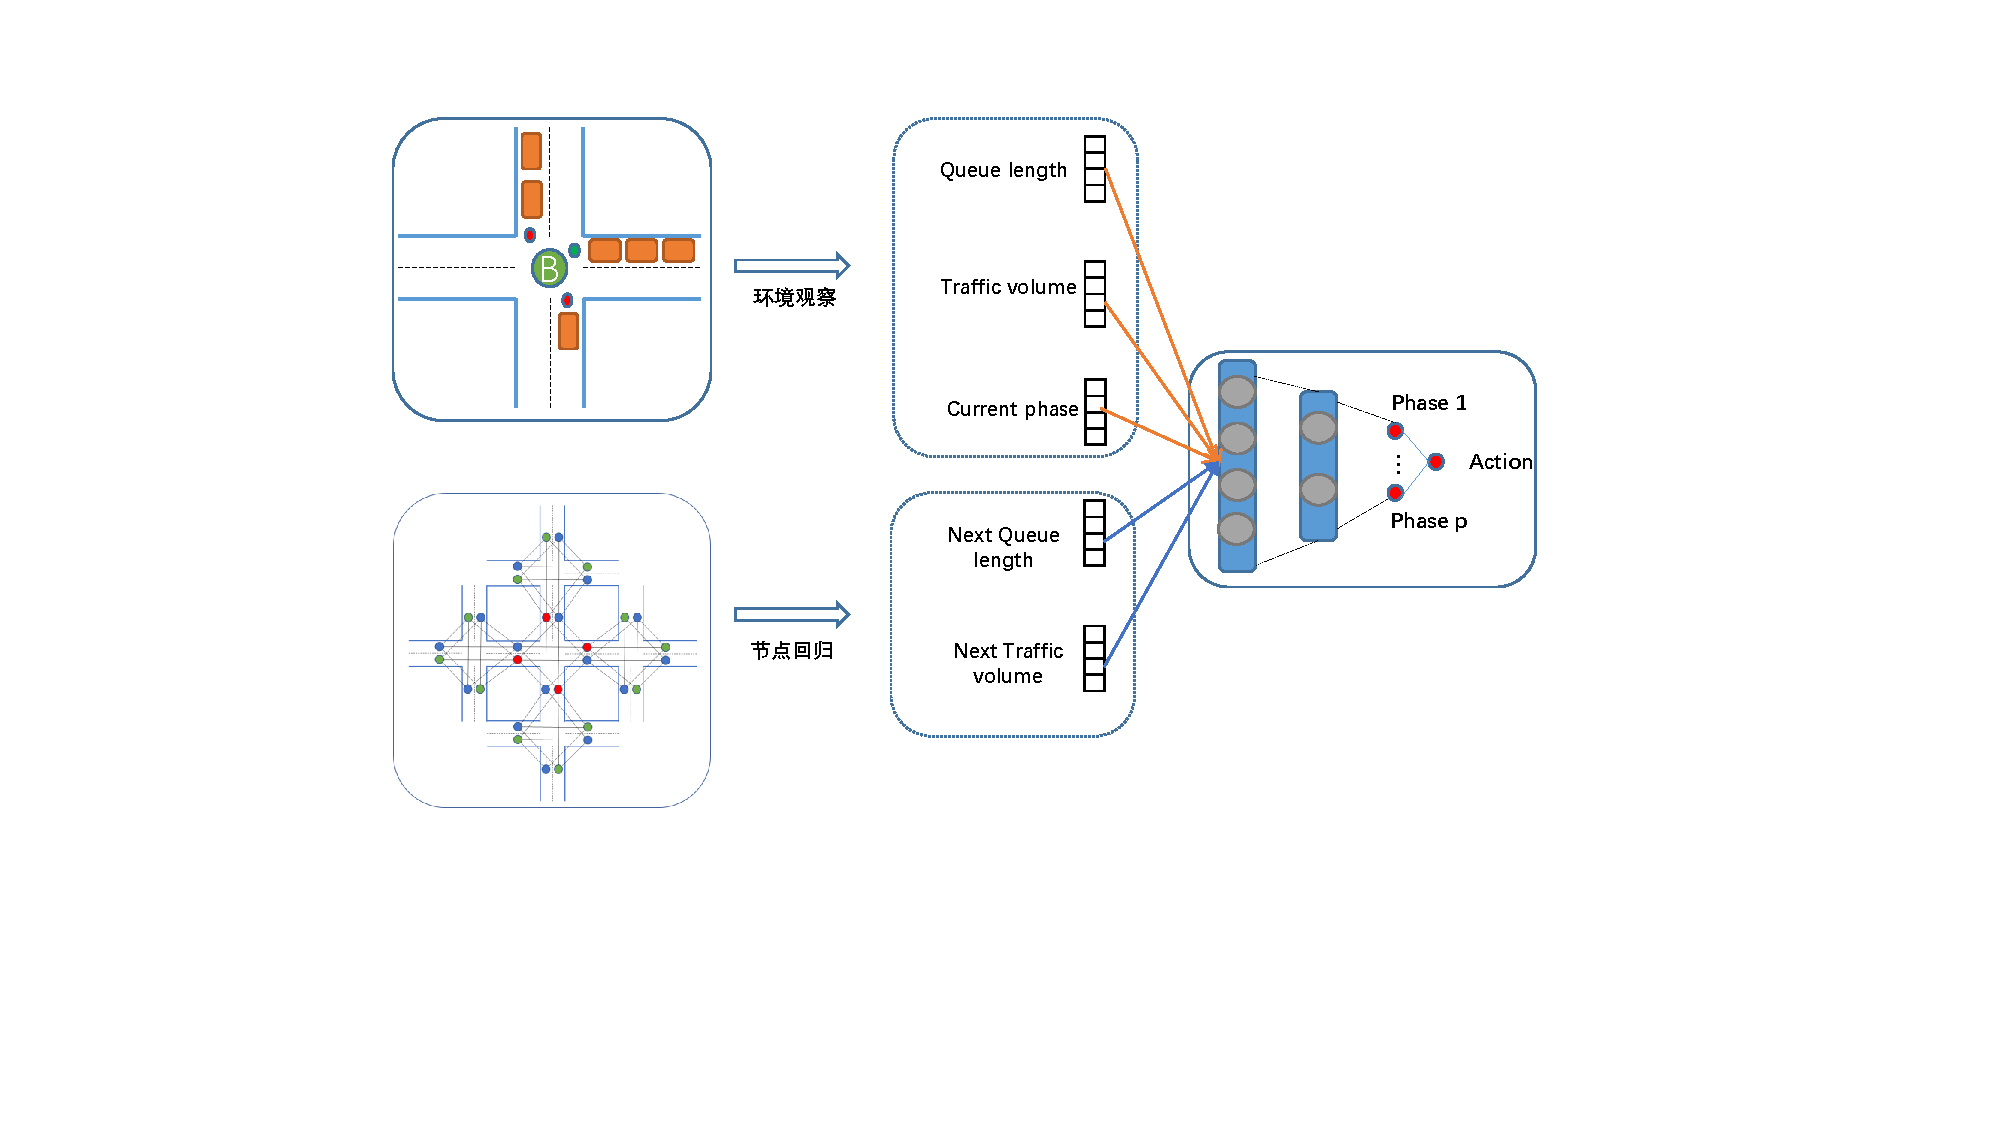
\includegraphics[width=0.9\textwidth]{fig/model-framework.pdf}
  \caption{模型框架}
  \label{fig:model-framework}
\end{figure}
\section{实验}
我们分别在两个合成的数据集和两个真实数据集上对我们的方法进行了实验,以评估我们方法的性能。由于实验是对针对多路口场景,我们这里的仿真工具使用的是CityFlow\footnote{http://cityflow-project.github.io},其对大规模交通信号控制的支持更加出色。
\subsection{数据集介绍}
\textbf{合成数据:}延用\inlinecite{wei2019colight}的做法,我们使用了以下以下两种人为合成的交通数据:
\begin{itemize}
  \item $Grid_{6x6}-b$:6x6的路网结构,其中每个路口有四个方向(西$\rightarrow$东、东$\rightarrow$西、南$\rightarrow$北以及北$\rightarrow$南),每个方向有三条车道(长300米,宽3米)。车辆在西$\leftrightarrow$东方向的生成速率是300辆/车道/小时,在南$\leftrightarrow$北方向的生成速率是90辆/车道/小时。
  \item $Grid_{6x6}$:与$Grid_{6x6}$的路网结构相同,但是只有单向的车辆流动,即只有西$\rightarrow$东和北$\rightarrow$南的单向交通流动。
\end{itemize}
% 在合成道路网中,每个路口有四个方向(西\rightarrow东、东\rightarrow西、南\rightarrow北以及由北\rightarrow南),每个方向有三条车道,每条车道长300米,宽3米。

\textbf{真实数据:}我们还使用了杭州和济南两个城市某个路段下采集到的真实数据\footnote{https://traffic-signal-control.github.io/\#open-datasets}进行了实验,\autoref{tab:real-world-datasets}统计了这两个数据集的关键信息。
\begin{table}[htb]
  \caption{数据统计}
  \label{tab:real-world-datasets}
  \begin{tabular}{lccccc}
  \toprule
  \multirow{2}{*}{数据集} & \multirow{2}{*}{路口数量} & \multicolumn{4}{c}{车辆到达率(300辆/s)} \\
  & & \multicolumn{1}{c}{均值} & \multicolumn{1}{c}{方差} & \multicolumn{1}{c}{最大值} & \multicolumn{1}{c}{最小值} \\
  \midrule
  $D_{Hangzhou}$ & 16 & 526.63 & 86.70 & 676 & 256 \\
  $D_{Jinan}$ & 12 & 250.70 & 38.21 & 335 & 208 \\
  \bottomrule
  \end{tabular}
\end{table}
\begin{itemize}
  \item $D_{Hangzhou}$:这个数据集中有16个路口,其中交通数据是由路侧监控摄像头拍摄产生,每条数据包含时间、摄像头ID和车辆信息。通过使用摄像头位置分析这些记录,记录车辆通过道路交叉口时的轨迹。我们以通过这些路口的车辆数作为实验的交通量。
  \item $D_{Jinan}$:与$D_{Hangzhou}$类似,数据集中包含了12个路口。
\end{itemize}:

\subsection{比较方法}
我们将我们的方法与传统交通控制方法和基于强化学习的几种方法进行了对比:
\begin{itemize}
  \item FT\cite{koonce2008traffic}: 这种方法以预先设定的方式循环改变信号。
  \item MaxPressure\cite{varaiya2013max}:传统交通领域最先进的网络级的交通信号控制方法,每次调度时,选择压力最大的相位。
  \item Individual RL\cite{wei2018intellilight}:一种基于深度强化学习的交通信号控制方法,不考虑邻居信息。每个路口由一个智能体控制,智能体之间不共享参数,而是独立更新自己的网络。
  \item GCN\cite{van2016coordinated}:一种基于深度强化学习的交通信号控制方法,使用图卷积神经网络(GCN)提取相邻路口的交通特征,不过其图建模方式是以路口为节点。
  \item Colight\cite{wei2019colight}:与GCN方法类似,都是以路口为节点的图建模方法,不过其使用GAT来学习不同路口之间的动态交互。
  \item GAT-Road:我们的方法,基于一种新的图建模方式(以道路为节点)。
\end{itemize}
\subsection{性能表现}

\begin{table}[htb]
  \caption{不同方法在合成数据集和真实数据集上关于平均通行时间的表现}
  \label{tab:performance}
  \begin{tabular}{lcccc}
  \toprule
  方法 & $Grid_{6x6}-Uni$ & $Grid_{6x6}-Bi$ & $D_Hangzhou$ & $D_Jinan$ \\
  \hline
  Fixedtime & 209.68 & 209.68 & 728.79 & 869.85 \\
  MaxPressure & 186.07 & 194.96 &  422.15 & 361.33 \\
  \hline
  Individual RL & 314.82 & 261.60 & 345.00 & 325.56 \\
  GCN & 205.40 & 272.14 & 768.43 & 625.66 \\
  CoLight & 173.79 & 170.11 & 297.26 & 291.14 \\
  \hline
  GAT-Road & \textbf{156.32} & \textbf{161.56} & \textbf{290.44} & \textbf{279.67} \\
  \bottomrule
  \end{tabular}
\end{table}
我们在合成数据和真实数据上进行了大量实验,并和已有方法进行了对比,然后在通行效率和模型收敛性上进行了分析。

\subsubsection{性能比较}

\textbf{效率比较}:
\autoref{tab:performance}列出了所有方法在合成数据和真实数据上路口的平均通行时间,可以看出,无论是在合成数据还是真实数据集上,我们的方法都取得了最好的表现。进一步的观察数据我们可以看出:
与传统交通控制中最先进的方法(MaxPressure)相比,我们的方法在合成数据和真实数据上都取得了一致的性能改进,其中在合成数据上的平均改进率是$16.6\%$,在真实数据上的平均改进率是$26.9\%$。

在合成数据上,Fixedtime的表现相对比较出色,但是在真实数据上,和基于学习的方法的性能差异变得明显。这是因为人为合成的数据是相对比较规则的数据,车辆流动的随机性没有真实数据中强,交通相对更加稳定。

GCN在真实数据上的表现并不出色是因为其在聚合邻居节点的信息时,是根据预先定义的静态权重处理邻居节点的信息,而不是根据实时的交通情况进行动态调整,当面对到变化性较强的真实数据时,这种静态处理方式会导致无法正确地聚合信息。

虽然CoLight也是使用GAT学习邻居节点的动态交互,但是由于其是以路口为节点来进行建图的,在数据交互的时候传递的是路口的所有交通信息,导致目标节点在聚合信息时难以挖掘有效的信息。而我们的方法GAT-Road以道路为节点进行建模,并且根据相位信息剔除掉了对目标节点无效的信息,因此表现更加出色。

\textbf{收敛性比较}:
我们将我们的方法GAT-Road与其他三种基于学习的方法(Individual、GCN和Colight)分别合成数据和真实数据上的学习收敛速度进行了比较,结果如\autoref{fig:convergence}所示通过对比我们可以看出:
\begin{figure}[t]
  \subfloat[$Grid_{6x6}$]{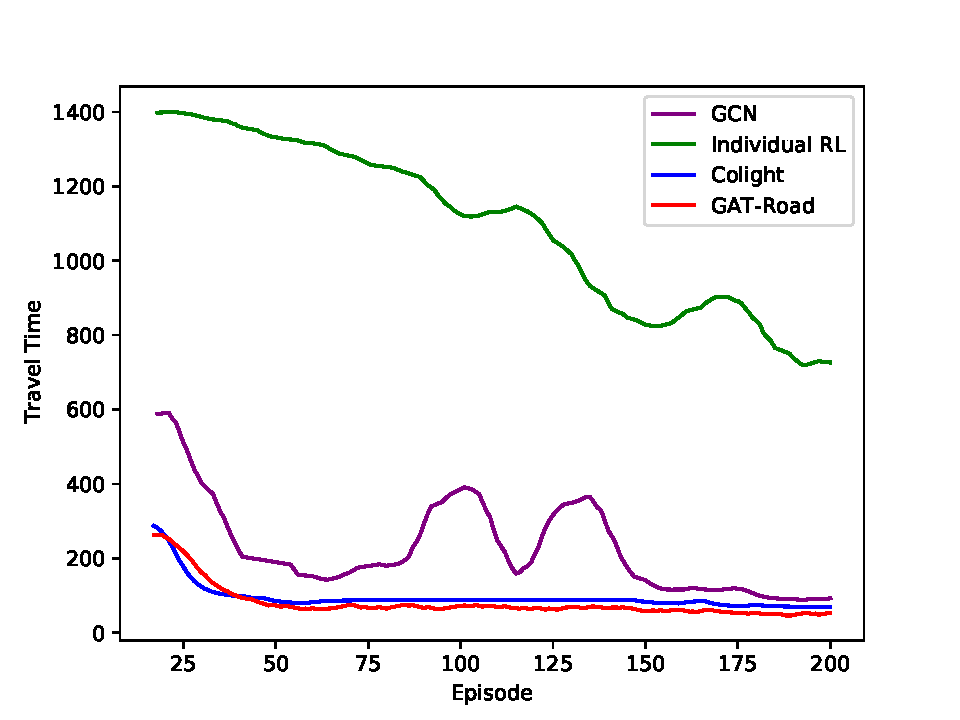
\includegraphics[width=0.45\textwidth]{./fig/conv-6x6.pdf}}\quad
  \subfloat[$Grid_{6x6}$-b]{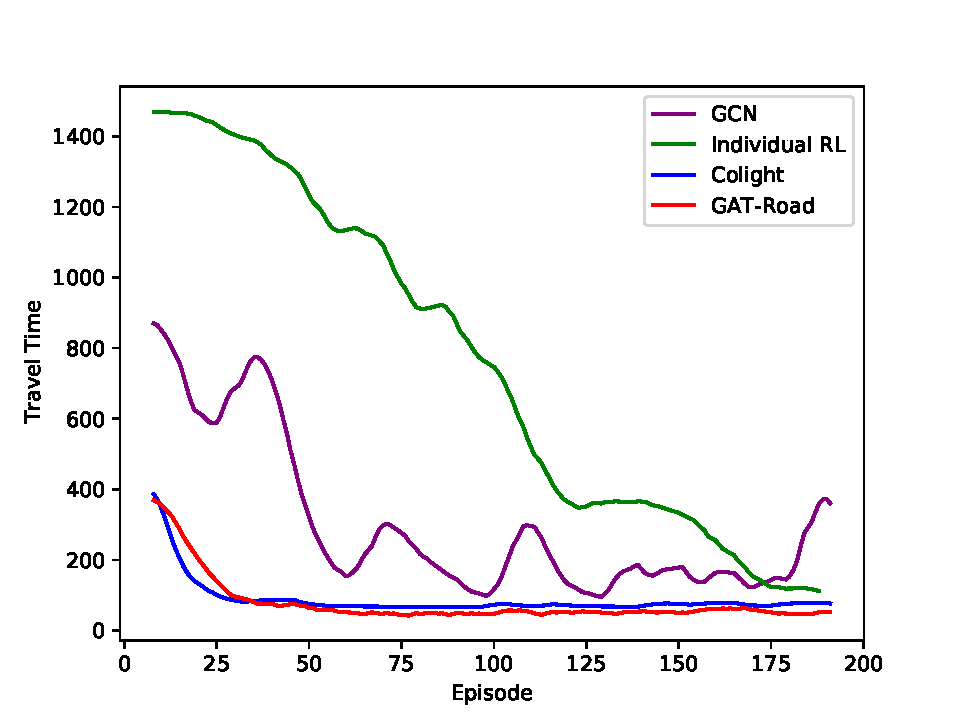
\includegraphics[width=0.45\textwidth]{./fig/conv-6x6-b.pdf}}\\
  \subfloat[$D_{Hangzhou}$]{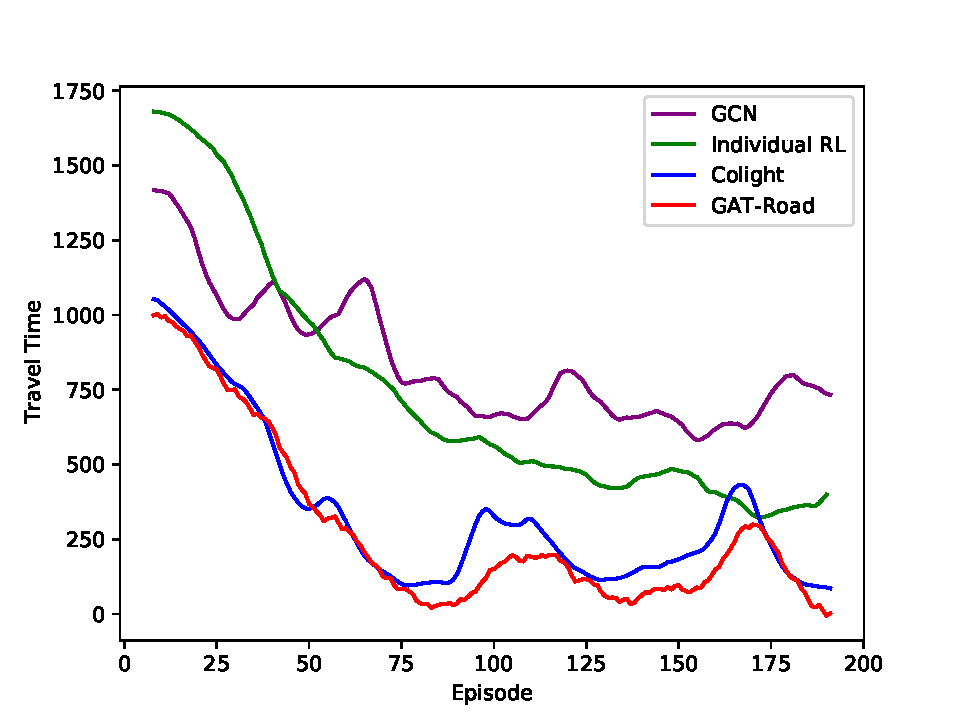
\includegraphics[width=0.45\textwidth]{./fig/conv-Hangzhou.pdf}}\quad
  \subfloat[$D_{Jinan}$]{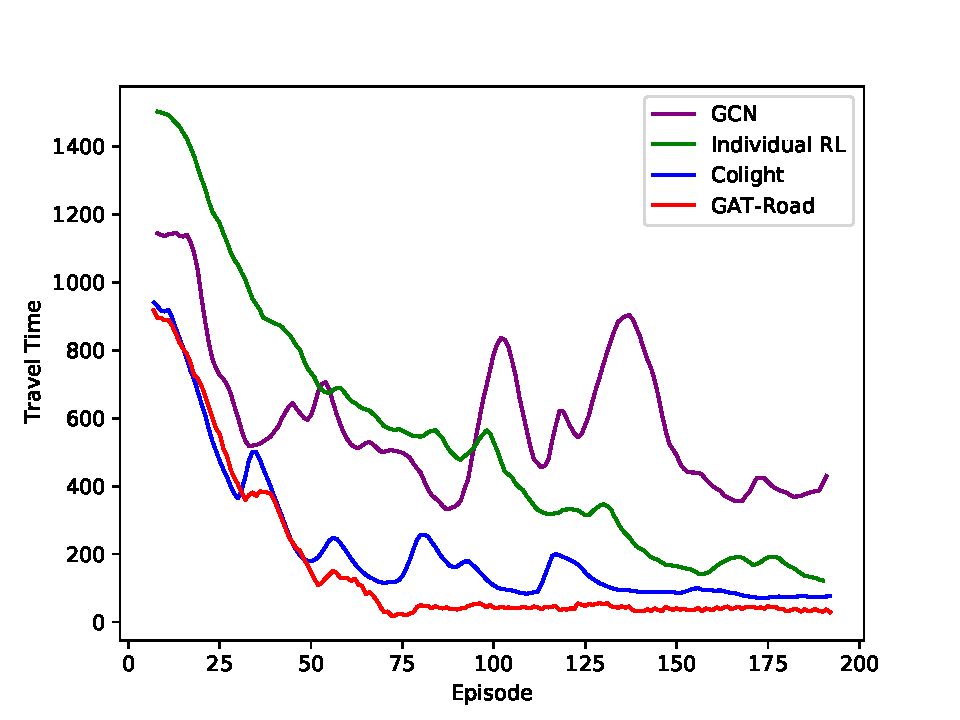
\includegraphics[width=0.45\textwidth]{./fig/conv-Jinan.pdf}}
  \caption[]{GAT-Road和其他三种基于学习的方法的收敛速度}
  \label{fig:convergence}
\end{figure}
与同样是使用IRL with Communication框架的GCN和Colight相比,我们的方法的收敛速度更快,这得益于我们提出的新的建图方式,在这种建图方式下,节点在进行信息聚合时可以剔除与目标节点无关的信息,从而降低了学习的难度,模型更容易收敛。

GCN方法在合成数据上收敛效果较好,但是在真实数据上收敛效果差的原因和上一节效率结果分析中的一样,静态的处理邻居路口的交通导致其难以聚合准确的信息。

虽然Individual最终也能收敛到最佳性能,但是由于其是独立优化单个路口的策略,没有考虑到周围路口环境的交通信息,因此其刚开始时的性能表现相较于其他三种方法更差,并且收敛速度更慢。


\section{本章小结}
\chapter{总结与展望}
\section{工作总结}
本文主要研究了基于深度强化学习的智能交通信号调度问题,包括单路口场景以及多路口场景下的信号调度问题。首先我们总结了一些传统的交通信号控制方法,这些方法要么受制于一些严苛的假设条件导致难以应用于实际交通控制中,要么缺乏对实时交通状况的考虑导致无法高效地缓解交通拥堵的情况。
然后我们总结了一些已有的使用深度强化学习解决智能交通信号调度问题的工作,在不同的调度场景下(单路口场景和多路口场景),我们对这些已有工作的进行了系统的分析,并指出他们存在的不足,最后我们针对这些不足提出新的解决方案。

对于单路口场景下的交通信号控制,已有的基于学习的方法更多的注重于提高通行效率,而忽略了公平性问题。在本文中,我们提出了一个新的模型可以在保证通行效率的同时,兼顾到对公平性的考虑。最后,我们在仿真环境中进行了大量的实验来验证我们模型的效果,并与已有方法进行对比,进一步阐述了我们模型在公平性方面的性能提升。

对于多路口场景下的交通信号控制,我们使用了IRL with communication的协调控制框架,并提出了一种新的将道路网建模成图的建模方式,在此基础上,我们设计了一种新的信息交互模块,通过这个信息交互模块,智能体在提取邻近节点的信息时可以剔除那些对自己无用的信息。最后我们在仿真环境中分别就合成交通数据和真实交通数据进行了实验,并与已有方法进行对比,进一步阐述了我们的模型在通行效率和学习速度上的提升。

\section{未来展望}
虽然目前有很多使用强化学习来解决智能交通信号调度的工作,并且也取得了不错的效果,但是任然有一些问题值得被深入研究:

\textbf{(1)信用分配问题}

信用分配问题是强化学习领域中被广泛研究的问题之一,它考虑的是对一个动作的成功(或失败的惩罚)的信用分配,即一个动作对于最终任务的实现有多大的贡献度,或者对于最终任务的失败应该承担多大的责任。在交通信号控制问题中,交通状况是交通信号控制器所采取的若干行动的结果,这带来了两个问题。(1)一个行动可能在几步行动后仍有效果;(2)每个时间戳的奖励是之前几个动作的组合结果。
在常规的强化学习应用环境中(例如,Atari游戏或围棋),有时会把一个训练集的最终得分分配给与这一集相关的所有动作,而交通信号控制问题中的动作从执行到产生影响可能有一个时间间隔,这个时间间隔可能是动态变化的,需要进一步研究。

\textbf{(2)Bus-Priority问题}

Bus-Priority是指在交通信号调度中,公共交通车辆相较于普通车辆应该具有更高的调度优先级,以鼓励人们在日常出行中乘坐公共交通用具。但是目前很多工作为了简化控制难度,都是无区别的对待道路上的交通流量。

\textbf{(3)实地测试问题}

目前有很多使用强化学习来解决智能交通信号调度的工作都只停留在仿真阶段,即实验场景的搭建以及效果的验证都是通过仿真器完成的,要想将这些模型部署到现实生活中的信号灯上还需要更多的研究和实地测试。但是随着车联网技术的发展使得我们可以实时地获取道路上车辆的信息,加上最近人工智能技术的崛起,
一些基于学习的交通信号调度算法可以在与环境的交互中不断的提升自身的性能,这些因素为进一步实现真实道路场景下的智能交通信号控制提供了技术支持。

\textbf{(4)安全性问题}

如何使强化学习智能体在物理环境中可以被接受是未来研究的一个重要方向。虽然强化学习方法从试错中学习,但在现实世界中,学习成本可能是关键的,甚至是致命的,因为交通信号的故障可能导致很严重的事故。因此,如何在强化学习中采用风险管理从而防止在智能体的学习过程中和学习结束后出现不必要的行为是十分关键的问题。



\appendix
% 如果需要附录的话,在这里 include
% \chapter{后记}

\section{v0.9a后记——Old Jack 的吐槽}

\verb!\begin{轻松+愉快}!

Old Jack 他有点累......

Old Jack 两年前就开始关注南航毕设的\LaTeX 模板了,但是两年了还没有任何有实际意义的新动作,所以Old Jack 就亲自操刀制作了新的一版。虽然很多代码都是从其他模板中直接摘抄过来的,但是这也是\TeX 最普遍、最快捷的学习\&开发方法。一开始 Old Jack 也想造轮子,但是轮子真的不好造。

在制作过程中遇到了几个关键性的问题:
\begin{itemize}
  \item 前文提到的三种粗体
  \item nuaa.png源文件和页眉制作
  \item 英文字母、章节标题莫名其妙的加粗
  \item 脚注相对页脚线的位置
\end{itemize}

第一个问题 Old Jack 曾经用\TeX 中伪粗体(FakeBold)的方法实现过,但是效果并不好,而且当时受到最后一个问题的强烈影响,不得不使用其他字体来解决这个问题。

第二个问题 Old Jack 开始是使用官方模板中的图片,但是分辨率太低,效果很差。于是 Old Jack Google以图搜图找到了现在的这个文件的源文件,经过了一系列不可描述的操作后得到了现在的 nuaa.png 。页眉的制作也让 Old Jack 很头疼,论文要求论文到顶端和底端的距离分别为2.5cm和2.0cm,Old Jack 很naive的就给geometry设置了这个数值,但是效果和官方模板差了很多,于是 Old Jack 只好一点一点地调试,达到了近似官方模板的效果。页脚和官方模板有细微的区别,Old Jack 认为这无伤大雅,是要罗马数字和阿拉伯数字编号正确应该就可以了。

第三个问题是一个非常奇怪的问题。使用伪粗体时所有标题全都加粗了,非常难看,经过了代码重构和不停地调试解决了这个问题。在模板完成99\% 后发现最后致谢中的英文字体全都加粗了, Old Jack 几次审视代码和调试都没有解决。偶然间,Old Jack 将全部主要文件全部提取出来,放入另一个文件夹,然后重新编译就解决了这个问题!当然后来发现代码中确实有一个地方有小问题\textbf{可能}会影响,但是这不是上一次出错的原因。Old Jack 对于各位使用模板的南航学子以及其他可能会参考此模板的\TeX 爱好者提了一个建议:\textbf{任何语言,任何代码出现莫名其妙的问题时,换一个文件夹,改一下名字,重新跑一下,可能会得到意想不到的结果。}当然这不是万能的解决方法。

第四个问题就如第一章中脚注和页脚线的情况,感觉两条线很别扭。 Old Jack 犹豫了很久,最后没有采用将脚注放在页脚线下的方案,因为 Old Jack 觉得还是两条线的方案好看。对于想要将脚注放在页脚线下方的同学,可以在主文件中取消注释那段代码,来实现所需要的效果。

Old Jack 他完成了模板的再制作,但是他没有心气再写出一篇能够指导大家使用\LaTeX 的文档了(好吧,Old Jack 他承认懒是一部分因素),望大家谅解 Old Jack。

\verb!\end{轻松+愉快}!

\section{v1.0后记}

Old Jack 非常高兴,因为他不是一个人在战斗。再次感谢张一白、王成欣、曾宪文、Gavin Lee等人的工作,没有他们,\nuaathesis 不会像现在这么美丽。

经过\nuaathesis~Group的努力和测试,\nuaathesis 迎来了v1.0版,也就是第一个正式发行版。一路走来也是有些坎坷,各种各样的小问题一直困扰着我们,其实v1.0 也还有着一些细小的问题尚未解决。不过Old Jack请大家放心,这些小问题不影响模板的使用。很多已经被我们解决的小问题比如页眉的大小位置,中英文字体是否正确,摘要的章节标题不能是加粗的宋体等等,老师可能不去管这些,甚至注意不到有什么区别。相比之下,重要的地方是:公式、图表的编号,图表和文本的位置,参考文献的格式等等才是老师关注的点。很多地方只是我们几个人为了追求和office模板尽可能接近,才不断地进行修改调整,也是有点讽刺。

写毕设论文的时候,Old Jack 不止一次看到隔壁室友调公式内容,Mathtype和Office装了卸,卸了装、调公式编号、调标题位置和大小、调首行缩进、调段间距等等等等,看着他们搞得焦头烂额的,Old Jack 都觉得心累。打印时也是这样,有太多的人在打印店不停地修改自己的论文,有因为office和wps不兼容修改的,有office版本不兼容修改的,有因为页眉页脚错误修改的等等。然而 Old Jack 他在写论文时从来没有担心过这些事情(当然,作为模板开发者 Old Jack 确实操心了很多,2333),他也第一次真正体会到了什么叫做专注于内容,真的挺轻松的(表格是例外)。

对于模板的推广,Old Jack觉得使用人数仍然不会太多,毕竟\LaTeX 的群众基础太小,除了8院,其他学院对公式的需求整体来讲并不迫切,Old Jack 猜测大部分知道、了解\LaTeX 的同学是通过数学建模竞赛这个途径才学习了\LaTeX ;同时因为涉及到学习新的程序语言,时间成本也较大,所以很多同学的学习意愿不高。不过\nuaathesis 的目标人群本来也不是全校所有学生,Old Jack 的思路,Old Jack 相信也是\nuaathesis~Group其他开发者的思路是:
\begin{enumerate}
  \item 为自己服务,这是\nuaathesis~Group开发模板的第一动力;
  \item 对已经掌握\LaTeX 基本语法的同学,\nuaathesis~Group为他们在毕业设计时能更轻松地撰写论文,提供平台和机会;
  \item 对准备学习\LaTeX 以及已经学习了一点\LaTeX 的同学,\nuaathesis~Group为他们提供学下去的动力和平台。
\end{enumerate}

即将毕业了,回首大学四年, Old Jack 做过疯狂的事情,也找到了一份看起来还可以的工作,只觉得还没对学校做过什么有用的事情,尽管 Old Jack 对学校其实并不是很有感情。完成了这个模板后,至少 Old Jack 可以减少一个遗憾,然后离开学校了。虽然这不是什么惊天动地的工作,但是至少 Old Jack 做了件他认为还算有意义的事情。Old Jack应该还会再维护\nuaathesis 一段时间,期待有后继者能够接过火炬,继续完善并推广\nuaathesis 。

想说的可能也就这么多了,Old Jack out!

\hfill 0813~王志浩,2017.6.24

\section{v2.0 后记 by yzwduck}

也是两年前开始关注南航毕设的\LaTeX 模板了,但直到毕业前,都没能去静下心来学习\LaTeX。

现在差不多本科毕业一年,或者说,一年后要开写硕士学位论文了,
本打算照着 CQUThesis 来造轮子的时候,逛纸飞机\footnote{论坛还活着吗?该不会已经沦落为老人的回忆了吧。 ——2018.10.10}
看到 \nuaathesis~v1.0 发布了。
非常激动、也很自愧,同样是经历了大学四年的人,我没能把这模板做出来。

于是马上把两年前为了模板而画的校名(矢量图)传了上去\footnote{\url{https://github.com/nuaatug/nuaathesis/commit/24fa82e}}。

原本打算在 v1.0 版的基础上修改的,但因为行间距设置有问题,封面与 Word 模板也有点差异,
还要再加入硕/博士的模板,于是干脆改成 \texttt{Documented LaTeX Source (.dtx)},
方便以后写模板的文档。

做模板过程中遇到的大问题,在于如何正确理解学校对论文格式的要求。
虽然有《本科毕业设计(论文)撰写格式要求》、《研究生学位论文撰写要求》,
但这些要求依然不够细致,因为那些要求都是假定你用 Word 来写论文的,要求里的内容是 Word 设置的操作方法,
所以还要先学习 Word 的排版算法。虽然这不是热门的资料,而且还有 CJK 独有的坑,
幸好有人把 Word 排版算法解释得非常详细,这个模板才能避免大量使用测量得到的魔数。
但还有很多细节部分,因为能力有限,没能实现。

最后容我吐槽一下学校的 Word 模板,我觉得那个 Word 模板可能从最初做出来后,就基本没有变化。
那个“最初”或许可以追溯到上个世纪。很多编号的事情都要由手工来完成,比如说目录页码、
各级标题的编号、题注等。这些完全可以自动编号的工作,如果要手工做的话【掀桌颜文字】。

\section{v2.1 后记 by yzwduck}

转眼间一年过去,又到了写毕业论文的时候了。

翻了一下代码的 commit 记录(部分非公开),这一年间只有加起来两、三个星期在做这个论文模板,
已经无法用“懒”这字来描述鄙人的状态了。

不过也有几件值得小小炫耀一下的事,终于把中/英/日多国语的坑填了不少,至少能编译出对应语言的论文来;
为了减少重复代码,使用一些宏包造了 \CTeX{} 的几个轮子,从而实现一个 class 文件能支持三国语言。

为了检验模板的效果,鄙人从知网上找了两篇论文,试着用 \nuaathesis{} 模板排版了一下(节选),又发现了不少问题。
因此目前 \nuaathesis{} 应该还有相当多的问题的,但没有用户的话,由于鄙人能力有限,难以发现,
还请各位使用 \nuaathesis{} 的先行者们(Pioneers) 能反馈意见和建议。

愿所有使用 \nuaathesis{} 的人,不会被评审老师指责格式问题。


\backmatter
% 如果参考文献使用 biber
\bibliographystyle{nuaabib}   % 参考文献的样式
\bibliography{bib/ref}   % 参考文献,即 bib/sample.bib 文件(纯文本)
% 如果打算手写参考文献
% \chapter{\bibname}

\begin{manref}
\item \label{ref:hint} 本节演示如何手写参考文献目录
\item 如果论文能用 biber 来管理参考文献的话,请使用 biber,不要手写
\item 如果实在不方便用 biber 的话,可以使用这种方法来手写参考文献。格式完全手写会有点繁琐,而且不能在正文中引用。比如:
\item \label{ref:man} KANAMORI H. Shaking without quaking[J]. Science, 1998, 279(5359): 2063.
\item 吴云芳.面向中文信息处理的现代汉语并列结构研究[D].北京:北京大学,2003[2013-10-14].
\end{manref}

示例:[\ref{ref:hint}] 这种写法不符合学校的要求,推荐使用这种写法\mcite{ref:man}。


\chapter[致谢]{致\hskip\ccwd{}谢}

在此感谢对本论文作成有所帮助的人。

\chapter{在学期间的研究成果及学术论文情况}

% 不要在意为什么没有 section,因为只是套用一下格式

\subsection*{攻读硕士学位期间发表(录用)论文情况}

\begin{enumerate}
  \item 以后可能会在这里也用上 biber
  \item 不过目前还需要手写论文全称
\end{enumerate}

\subsection*{研究生期间参与的科研项目}

\begin{enumerate}
  \item 国家自然科学基金 (No.12345678)
\end{enumerate}


\end{document}
